%\documentclass[a4paper,12pt,final]{report}
% Pour une impression recto verso, utilisez plutôt ce documentclass :
\documentclass[a4paper,11pt,twoside,final,openany]{report}
%\documentclass[a4paper,12pt,oneside,final]{book}
%\documentclass[a4paper,12pt,oneside,final]{book}


%\usepackage[english,francais]{babel}
\usepackage[francais]{babel}
\usepackage[utf8]{inputenc}
\usepackage[T1]{fontenc}
\usepackage[pdftex]{graphicx}
\usepackage{setspace}
%\usepackage{hyperref}
\usepackage[hidelinks]{hyperref}
\usepackage[french]{varioref}
%\usepackage[left=2cm,right=2cm,bottom=1.8cm,top=2cm]{geometry}
\usepackage[bottom=2.0cm,top=2.5cm]{geometry}
%\usepackage{geometry}
 \usepackage{float}

\usepackage{amssymb}
\usepackage{amsthm}
\usepackage{fancybox}
\usepackage{amsmath}
\usepackage[french,ruled,scleft]{algorithm2e}
\usepackage{fancyhdr}

\usepackage{shorttoc}

%\RequirePackage[hyperpageref]{backref}
%\backreffrench 

\usepackage[babel,french=guillemets*]{csquotes}
\MakeOuterQuote{"}

\newsavebox{\auteurbm}
\newenvironment{extrait}[1]{\small\slshape
	\savebox{\auteurbm}{\upshape\sffamily#1}
	\begin{flushright}}{\\[4pt]\usebox{\auteurbm}
	\end{flushright}\normalsize\upshape}


\usepackage[active,tightpage]{preview}

\usepackage{stmaryrd}

\usepackage{tikz}
\usepackage{pgf}
\usetikzlibrary{matrix}
\usetikzlibrary{calc}
\usetikzlibrary{fit}
\usetikzlibrary{arrows,automata}
\usetikzlibrary{automata,positioning}
\usetikzlibrary{shapes.multipart}

\tikzstyle{every loop}=[->,shorten >=1pt,looseness=8]
\tikzstyle{loop below}=[in=-100,out=-80,loop]
\tikzstyle{loop above}=[in=100,out=80,loop]


\newcommand{\reporttitle}{Analyse de faisabilité d'une mission par calcul de trajectoire sous contraintes de stabilité}     % Titre
\newcommand{\reportauthor}{M.~Romain \textsc{Pichard}} % Auteur
\newcommand{\reportsubject}{Stage de fin d'étude} % Sujet
\newcommand{\HRule}{\rule{\linewidth}{0.5mm}}
\setlength{\parskip}{1ex} % Espace entre les paragraphes

\hypersetup{
    pdftitle={\reporttitle},%
    pdfauthor={\reportauthor},%
    pdfsubject={\reportsubject},%
    pdfkeywords={rapport} {vos} {mots} {clés}
}

\theoremstyle{plain}
\newtheorem{theo}{Théorème}

\theoremstyle{definition}
\newtheorem{definition}{Définition}

\theoremstyle{remark}
\newtheorem{rem}{Remarque}

%\pagestyle{headings}
\pagenumbering{arabic}

\pagestyle{fancy}


\makeatletter
\def\@makechapterhead#1{%
	\vspace*{20\p@}%
	%\vspace*{-1cm}%
	{\parindent \z@ \raggedright \normalfont
		\interlinepenalty\@M
		\Huge \bfseries\thechapter.\quad#1\par\nobreak
		\vskip 20\p@
	}}
	\makeatother

\renewcommand \thechapter{\Roman{chapter}}
\renewcommand \thesection{\arabic{section}}
\renewcommand \thesubsection{\arabic{section}.\arabic{subsection}}

\setcounter{secnumdepth}{3}
\setcounter{tocdepth}{3} 



\renewcommand{\headrulewidth}{1pt}
%\fancyhead[C]{\textbf{page \thepage}} 
\fancyhead[L]{\leftmark}
%\fancyhead[R]{\textbf{page \thepage}}
\fancyhead[R]{\rightmark}

\renewcommand{\footrulewidth}{1pt}
\fancyfoot[C]{\textbf{page \thepage}} 
\fancyfoot[L]{Romain Pichard}
%\fancyfoot[R]{\leftmark}

\begin{document}
  % Inspiré de http://en.wikibooks.org/wiki/LaTeX/Title_Creation

\begin{titlepage}

\begin{center}

\begin{minipage}[t]{0.48\textwidth}
  \begin{flushleft}
    
\includegraphics [width=30mm]{images/logo_univ_tlse.png} \\[0.5cm]
  \end{flushleft}
\end{minipage}
\begin{minipage}[t]{0.48\textwidth}
  \begin{flushright}
    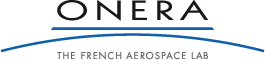
\includegraphics [width=50mm]{images/onera.png} 
  \end{flushright}
\end{minipage} \\[1.5cm]

\textsc{\Large \reportsubject}\\[0.5cm]
\HRule \\[0.4cm]
{\huge \bfseries \reporttitle}\\[0.4cm]
\HRule \\[1.5cm]

\begin{minipage}[t]{0.32\textwidth}
  \begin{flushleft} \large
    \emph{Auteur :}\\
    \reportauthor
  \end{flushleft}
\end{minipage}
\begin{minipage}[t]{0.6\textwidth}
  \begin{flushright} \large
    \emph{Responsables :} \\
    M.~Xavier \textsc{Pucel} \\
    M.~Thomas \textsc{Loquen}
  \end{flushright}
\end{minipage}

\vfill

{\large \today}

\end{center}

\end{titlepage}

 % \cleardoublepage % Dans le cas du recto verso, ajoute une page blanche si besoin
  %\shorttableofcontents{Sommaire}{1}
  \chapter*{Remerciements}
\addcontentsline{toc}{chapter}{Remerciements}
Au terme de mon stage je tiens à remercier toutes les personnes qui ont contribué à mes travaux et à ma vie pendant ces 5 mois à l'ONERA.

Je remercie mes encadrants : Xavier Pucel et Thomas Loquen qui ont su m'apporter leurs expériences et leurs conseils pour avancer dans les meilleurs conditions possibles lors de ce stage.

Je remercie également mes collègues de bureau, j'ai passé un très agréable moment en votre compagnie, merci pour vos soutiens et votre aide.

Je souhaite remercier l'ensemble des doctorants du DCSD pour leur accueil et leur gentillesse. Plus particulièrement, merci à Jéremy Lesprier, Adrien Maillard et Patrick Bechon pour avoir pris du temps sur leur rédaction de thèse pour m'aider et me débloquer dans les moments difficiles.  

Enfin, Léa, merci à toi de toujours être présente à mes côtés.
  %\addcontentsline{toc}{chapter}{Remerciements}  
  \tableofcontents % Table des matières
  \sloppy          % Justification moins stricte : des mots ne dépasseront pas des paragraphes
  
%\cleardoublepage



\chapter{Introduction}

\begin{extrait}{}
	Systèmes hybrides : systèmes faisant intervenir des phénomènes\\
	 de types dynamique continue et événementielle.
\end{extrait}

Actuellement, la planification de mission pour les systèmes de drone consiste à produire une séquence de points de passage, définis par leurs coordonnées, et associés à des actions à effectuer. Cette séquence définit un plan qui va être exécuté par les contrôleurs du drone. Avec cette démarche, l'aspect hybride de l'aéronef n'est pas, ou peu, prise en compte. En effet, la planification s'occupe de la mission dans son ensemble (contraintes géographiques, temporelles ...) et les contrôleurs assurent une commande garantissant la stabilité de l'engin et la réalisation du plan.

Les systèmes automatisés actuels, de par leur complexité ne peuvent plus être représentés uniquement par leur comportement continu ou leur comportement discret. De nombreux systèmes réels sont à dynamique continue, mais supervisée ou contrôlée par une dynamique discrète. La modélisation de ces systèmes nécessite une nouvelle approche et de nouveaux outils, c'est pourquoi ces dernières années de nombreux travaux vont dans ce sens et tentent de proposer des outils de modélisation et d'analyse.

Étant donné que la modélisation des drones évolue pour prendre en compte ces aspects hybrides, il parait logique que la planification se doit, elle aussi, de s'adapter et d'évoluer. 

%L'objectif de ce travail est de proposer une démarche et un outil de planification permettant la prise en compte de l'environnement de mission, ainsi que les contraintes intrinsèques d'un drone.

L'objectif de ce travail est de proposer une démarche et un outil de planification permettant de déterminer si un drone est capable de remplir une mission donnée, à partir d'une description formelle de la mission et d'un modèle de la dynamique du vol du drone.

De plus il est à préciser qu'il s'agit d'un travail exploratoire, le but est également de tester quels outils et méthodes, existants aussi bien en continue qu'en discret, peuvent contribuer à enrichir la résolution d'un problème de planification dans un cadre hybride.
\begin{center}
%	\noindent\rule{250pt}{.5pt}
\end{center}
\pagebreak
\chapter*{Organisation du manuscrit}
%Ce rapport suit l'organisation suivante : 

Le premier chapitre a pour but de présenter le contexte du stage via une présentation de l'ONERA qui m'a accueilli, mais aussi via une description plus détaillée de ma problématique de stage.

Le deuxième chapitre présente les différentes notions nécessaires à la compréhension de tous les domaines liés à notre problématique. En effet, la pluridisciplinarité du monde des systèmes hybrides nous oblige à introduire les aspects de stabilité de l'automatique continue mais aussi les méthodes de représentation issues des systèmes à événements discrets. Il est également présenté les différentes méthodes de planification existantes, et pour finir les démarches de planification spécifiques aux missions utilisant des drones.

Le troisième chapitre propose de résoudre notre problématique en utilisant un planificateur basé sur un problème de satisfaction de contraintes (CSP). Pour ce faire, la modélisation de l'environnement de mission ainsi que les contraintes de la dynamique du vol et du drone sont présentées.

Le quatrième chapitre présente l'implémentation de la démarche décrite au chapitre \ref{chapter:model} dans différents outils, ainsi que l'analyse des résultats obtenus avec chaque outil.

Le dernier chapitre apporte un bilan du travail effectué ainsi que les perspectives possibles.




 


\section{Cadre de travail à l'ONERA}
\subsection{Une entreprise historique}
L'ONERA - Office National d'Études et de Recherches Aérospatiales - est un organisme public de recherche pour les technologies aérospatiales. Il a été créé en 1946 pour accompagner le redémarrage de l'industrie aéronautique ravagée par la guerre. Depuis cette date, l'ONERA a contribué à tous les grands programmes aérospatiaux nationaux (Mirage, Concorde, fusées Diamant...) ou européens (Airbus, Ariane...). Son statut d'EPIC - Établissement Public à caractère Industriel et Commercial - lui assure une subvention étatique représentant environ 40\% de son budget annuel. Le reste provient d'une activité contractuelle, soit en son nom propre, soit au sein de consortium, pour les donneurs d'ordres variés (DGA, CNES, DASSAULT, ESA, UE, ANR...).

Ces travaux de recherche servent l'innovation et la compétitivité dans les secteurs de l'aéronautique, de l'espace et de la défense. Les missions de l'office sont de : 
\begin{itemize}
	\item Anticiper les ruptures technologiques pour \textbf{préparer l'avenir}
	\item Favoriser les \textbf{transferts vers l'industrie}
	\item Réaliser et mettre en œuvre des \textbf{moyens d'expérimentation et de simulation}
	\item \textbf{Fournir à l'industrie} des expertises de haut niveau
	\item \textbf{Expertiser pour l'État} les grands choix technologiques de demain
	\item \textbf{Former} des ingénieurs et des chercheurs
\end{itemize}

L'ONERA compte un peu plus de 2000 employés dont les trois quart sont des ingénieurs, techniciens ou doctorants. Son budget annuel dépasse les 220 millions d'euros.

Depuis Janvier 2007, pour répondre à une nécessité de visibilité internationale, le centre de recherche adopte la dénomination "ONERA : The French Aerospace Lab"

\subsection{La recherche à l'ONERA}
\textit{\textbf{La pluridisciplinarité des équipes}}

Les activités scientifiques sont organisées en 17 départements répartis en 4 branches scientifiques : 
\begin{itemize}
\item MFE : Mécanique des Fluides et Énergétiques
\item MAS : MAtériaux et Structures
\item PHY : PHYsique
\item TIS : Traitement de l'Information et Systèmes
\end{itemize}

L'ONERA est donc présent dans la plupart des disciplines scientifiques nécessaires aux progrès du secteur aérospatial. %En ce sens, il est déjà un organisme pluridisciplinaire. Mais il y a plus : ses chercheurs pratiquent au quotidien la fertilisation croisée des connaissances, en interne comme en externe. En réponse aux besoins de l'industrie, ils ont appris à travailler entre spécialistes de plusieurs disciplines, dans le cadre de projets à visées applicatives. Que ce soit entre équipes de l'ONERA, mais aussi avec d'autres, issues de laboratoires extérieurs.

\textit{\textbf{La dualité calcul-expérience}}

Les travaux de l'ONERA reposent sur une double approche : la simulation numérique et l'expérimentation. L'ONERA développe des codes de simulation numérique dans les différents domaines de l'aérospatial. Pour autant, l'expérimentation reste omniprésente, à chaque étape du processus d'acquisition des connaissances. Elle en est souvent le point de départ, sur des composants élémentaires dont on caractérise expérimentalement le comportement. Elle intervient ensuite, plus en aval, pour valider les modèles et recaler leurs paramètres sur des grandeurs physiques réelles.
 
\textit{\textbf{La connaissance des applications industrielles}}

En soixante-dix années de recherches menées pour le compte de l'industrie aéronautique, spatiale et de défense, l'ONERA a développé une tradition de confrontation avec l'application. Ses équipes ont tissé des liens avec les industriels et engrangé une somme inestimable de connaissances sur l'utilisation concrète de la science. Au final, les chercheurs sont en position d'anticiper les besoins de l'industrie et de proposer des solutions opérationnelles tenant compte de l'environnement applicatif.

\textit{\textbf{Un parc de moyens d'essais unique en Europe}}

%Pour mener sa double démarche Calcul/Expérimentation, l'ONERA dispose de trois catégories de moyens d'essais : premièrement les moyens d'essais de laboratoire

Pour mener sa double démarche Calcul/Expérimentation, l'ONERA dispose de trois catégories de moyens d'essais : premièrement les moyens d'essais de laboratoire comme les bancs de vélocimétrie laser, le canon à électrons... On trouvera également les moyens d'essais intermédiaires, c'est le cas de la maquette B20 à Lille, le banc de turbomachines aéronautiques Turma à Modane-Avrieux... Enfin les grandes souffleries dites "industrielles" du Fauga-Mauzac et de Modane-Avrieux constituent les grands moyens d'essais. Elles sont mises en œuvre, pour le compte de l'ONERA et pour des clients extérieurs, par une direction spécifique. Le parc de soufflerie de l'ONERA est le plus grand d'Europe.

\textit{\textbf{La dualité civil-militaire}}

L'activité de l'ONERA se répartit de façon équilibrée entre :
\begin{itemize}
	\item le civil
	\item la défense
	\item les recherches duales
\end{itemize}
Il est fréquent que des travaux initiés pour un secteur servent également à un autre par la suite.

\subsection{Départements d'accueil}

Mon stage s'est déroulé à l'ONERA Toulouse, dans le département DCSD - Commande des systèmes et dynamique du vol - de la branche TIS.

Les principaux champs d'actions du DCSD sont : 
\begin{itemize}
	\item Automatique
	\item Intelligence artificielle
	\item Robotique
	\item Conception et performances des systèmes aérospatiaux, cockpits et stations de contrôle
\end{itemize}

Le DCSD est lui même structuré en différentes unités de recherche. Mon stage s'est effectué en collaboration avec les unités CD - Conduite et Décision - pour ce qui est de la partie planification et automatique discrète, et CDIN - CommanDe et INtégration - pour ce qui est de la partie automatique continue et hybride.

\section[Problématique]{Position du problème et objectifs du stage}	
\noindent
\shadowbox{\begin{minipage}{\textwidth}
		\textbf{Résumé :} Le problème est de déterminer si un drone est capable de remplir une mission donnée, à partir d'une description formelle de la mission et d'un modèle de la dynamique du vol du drone. La méthode mise en œuvre implique des aspects de planification de commande, ainsi que de l'analyse de stabilité, et surtout l'intégration de ces outils. L'objectif est d'automatiser cette analyse le plus possible.
	\end{minipage}}
	
Dans le cadre de ce stage nous limiterons notre étude au problème longitudinal, c'est à dire que notre aéronef évoluera dans un espace 2D (distance et hauteur). Ceci nous permettra d'éprouver notre démarche sur un problème simple, puis par la suite d'étudier la faisabilité de notre démarche sur des déplacements longitudinaux et latéraux.

Les objectifs du stage sont multiples, tout d'abord il faut être capable de représenter mathématiquement un aéronef ayant des changements de modes de fonctionnement intrinsèques. Pour cela la démarche proposée est d'utiliser le formalisme des automates hybrides en considérant que chaque état de l'automate représente un mode de fonctionnement de l'aéronef (modélisé par un espace d'état linéaire).

Une fois que ce travail de modélisation de l'aéronef est effectué, il s'agit d'être capable de définir un environnement de mission et la mission, ceci dans le but de pouvoir planifier les commandes à appliquer à notre aéronef afin qu'il réussisse la mission. Tout ceci doit s'effectuer en garantissant la stabilité de l'aéronef.

Il est également à noter que ces travaux sont un préambule à différents projets futurs portant sur la planification des systèmes hybrides, nous devons déterminer les approches, outils, méthodes qui semblent être les plus pertinents pour résoudre ce type de problème.

L'environnement de la mission, c'est à dire le monde dans lequel l'aéronef va évoluer, peut se représenter sous la forme d'une coupe verticale de l'espace avec des zones interdites et des points de départ et d'arrivée. De plus la prise en compte des contraintes de stabilité de l'aéronef doit permettre d'éviter des scénarios dangereux, un exemple est présenté sur la figure \ref{fig:scenario} : 
%La zone rouge représente un nuage, la verte un couloir de navigation interdit et les bleu et jaune des montagnes. Les points de départ et d'arrivé sont également représenté.
\begin{figure}[!h]
	\centering	
	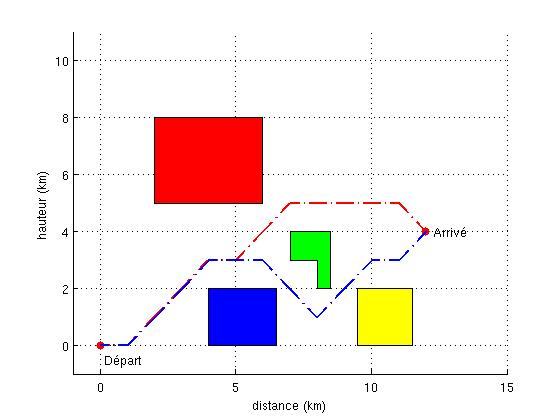
\includegraphics[scale=0.6]{images/scenario2.jpg}
	\caption{Environnement d'une mission}
	\label{fig:scenario}
\end{figure}

\pagebreak
Le scénario rouge semble respecter les contraintes de l'aéronef, en effet nous ne voyons pas de changement d'angle d'attaque trop élevé, en revanche, le scénario bleu présente un changement beaucoup trop brusque pour l'avion. Notre démarche doit donc permettre de fournir un scénario du type rouge.

%Nous faisons l'hypothèse que l'aéronef possède différentes lois de pilotage (monter, descendre, maintien, etc), chacune étant modélisée par un espace d'état linéaire (continu ou discret). L'interaction et les changements de loi de pilotage sont intrinsèques à l'aéronef et peuvent être représentés par un automate hybride.

Notre objectif est de proposer une démarche et des outils permettant la prise en compte d'un environnement, d'une mission et d'un aéronef présentant une dynamique hybride. La démarche doit être assez flexible et automatisée que possible, cela dans le but d'être appliquée à différents types d'aéronef et de mission.

Même si dans un premier temps l'exemple indiqué présente des aspects discrets limités qui peuvent être résolus manuellement, nous étudions des méthodes permettant de gérer des modèles dont la dynamique discrète est complexe (beaucoup d'obstacles, de points de passage, plusieurs avions/vols disponibles, etc...).

% comme présenté sur la figure \ref{exempleGraphe}.
%
%	\begin{figure}[!h]		
%		\centering	
%		\begin{tikzpicture}[->,>=stealth',shorten >=1pt,auto,node distance=2.8cm,
%		semithick,every text node part/.style={align=center}]
%		\tikzstyle{every state}=[fill=white,draw=black,text=black]
%		
%		
%		\node   (A)   at (2,1)  {};
%		\node[state]    (B)  at (3,0)     {mode 1 \\ maintien};
%		\draw[<-] (B) to[bend right] (A)  ;
%		
%		\node[state]    (C)   at (1,-3)     {mode 2 \\ monter};
%		\node[state]    (D)   at (5,-3)     {mode 3 \\ descendre};
%		
%		\path 
%		(B) edge [bend left=10] node {}   (C)		
%		(B) edge [bend right=10] node {}   (D)
%		
%		(C) edge [bend left=10] node {}   (B)		
%		(C) edge [bend left=10] node {}   (D)	
%		
%		(D) edge [bend left=10] node {}  (C)	
%		(D) edge [bend right=10] node {}  (B);		
%		\end{tikzpicture} 
%		\caption{Exemple d'automate hybride avec 3 lois de pilotage}
%		\label{exempleGraphe}
%	\end{figure}

%Une fois que nous avons le modèle de l'aéronef et que l'environnement de mission est établi, nous devons générer un plan répondant à la mission. Il faut s'assurer que ce plan ne va pas introduire d'instabilité sur l'engin. 

%Par exemple, sur la figure \ref{scenario} nous pouvons voir deux trajets répondant à la mission. Mais le trajet en bleu pose un problème car il imposerait des variations d'angle d'incidence entrainant un décrochage de l'aéronef.
%\begin{figure}[!h]
%\centering	
%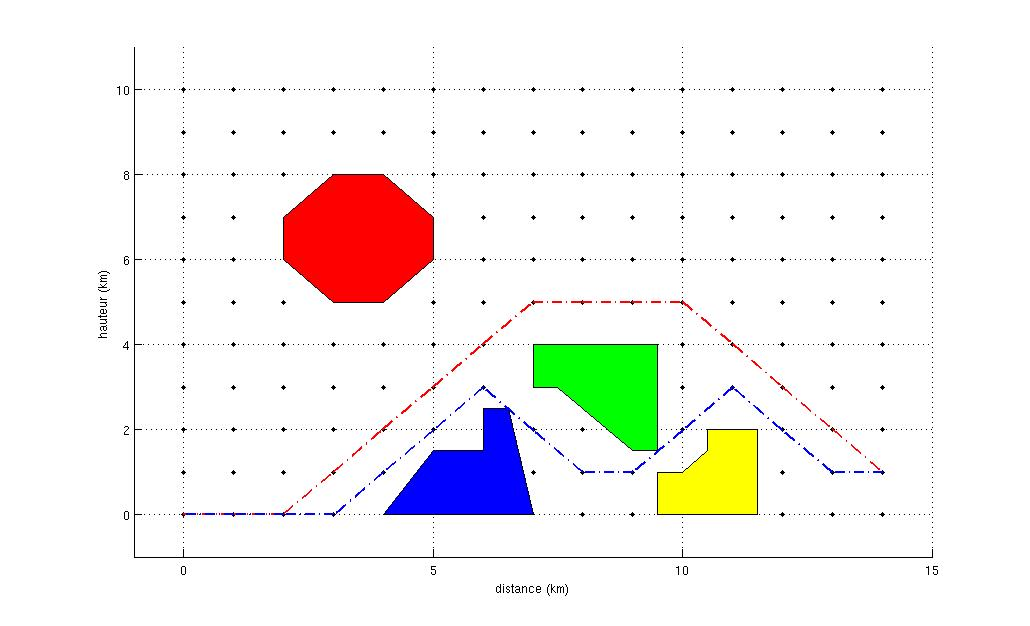
\includegraphics[scale=0.4]{images/scenario.jpg}
%\caption{Deux plans de mission (rouge : pas de soucis, bleu : décrochage possible)}
%\label{scenario}
%\end{figure}



\chapter{Bibliographie}
\section{Systèmes hybrides}

Cette partie a pour but de présenter les systèmes dynamiques hybrides, leurs problématiques, les différentes classes de systèmes hybrides ainsi que les différents outils de modélisation.
Nous nous appuierons fortement sur le travail de thèse de \cite{Kur02}, et plus particulièrement les parties 1.1 à 1.3. Étant donné que l'étude détaillée est faite dans ce travail de thèse, seule les idées principales sont reprises dans ce chapitre.

\subsection{Problématique}
Les systèmes automatisés actuels, de part leur complexité ne peuvent plus être représentés uniquement par leur comportement continu ou leur comportement discret, de nombreux systèmes réels sont à dynamique continue, mais supervisés ou contrôlés par une dynamique discrète. La modélisation de ces systèmes nécessitent une nouvelle approche et de nouveaux outils, c'est pourquoi ces dernières années de nombreux travaux vont dans ce sens et tentent de proposer des outils de modélisation et d'analyse.

\subsection{Classe de système hybride}
La nature hybride d'un système peut être inhérente aux phénomènes physiques qui le régissent, ou bien provoquée par une supervision de ce système. Il existe donc différentes classes de système hybride parmi lesquelles : 
\begin{itemize}
	\item \emph{Commutation autonome} : Caractérise un système qui va changer de façon discontinue lorsque l'état atteint certains seuils, c'est le cas des systèmes à hysteresis, la table de billard en est un exemple concret.
	\item \emph{Commutation contrôlée} : Traduit un phénomène où le système change de façon discontinue et instantanée en réponse à une entrée de commande, par exemple un système de thermostat. 
\end{itemize}

\subsection{Automate hybride}
La modélisation des systèmes dynamiques hybrides est un problème toujours en étude à ce jour \cite{goebel_hybrid_2012}. Le but est de réussir à trouver des outils permettant la représentation des dynamiques discrètes et continues dans une même syntaxe. L'automate hybride \cite{henzinger_theory_2000} est aujourd'hui un outil permettant de répondre à ces besoins. En effet, dans le domaine discret on représente très souvent les systèmes par un automate, en associant aux états des dynamiques continues, et en permettant aux transitions de dépendre elles aussi des conditions continues, il est possible de modéliser un système dynamique hybride.

\begin{figure}[h]
	\centering	
	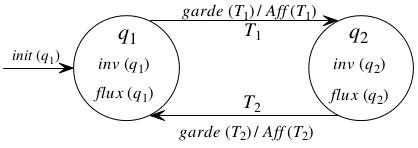
\includegraphics{images/automateHybride.jpeg}
	\caption{Automate hybride}
	\label{exempleAutomateHybride}
\end{figure}

L'\textit{état continu} du système est modélisé par un vecteur d'état continu $x(.)$ représentant un point dans un espace $X \subset \mathbb{R}^n$. Dans chaque sommet, la dynamique continue est modélisée par des conditions de flux telle que des équations différentielles ou des espaces d'états.

A chaque transition on associe un prédicat qui concerne l'état interne du système appelé \textit{garde}. Ce prédicat détermine les dates possibles pour le franchissement de la transition. Ainsi, une transition de l'automate hybride peut être franchie à l'instant $t$ si et seulement si sa garde est vérifiée par la valeur des variables d'état continues du système à l'instant considéré.

En général la garde d'une transition est exprimée par une région de l'espace d'état continu, qui peut se ramener à des intervalles.

L'ensemble des variables d'état continues mises à jour lors du franchissement d'une transition est décrit par une affectation. Les initialisations spécifiées par l'affectation correspondent à des fonctions, calculant la nouvelle valeur de l'état à partir de sa valeur avant le franchissement.

\begin{definition}{Un automate hybride d'ordre n, tel que présenté sur la figure \ref{exempleAutomateHybride} est défini par :}\\
\[\mathbb{A} = (Q, X, flux, inv, garde, Aff, init)\]
tel que :
\label{def:autom-hybride}
\begin{itemize}
\item Q = {$q_1, q_2, \ldots, q_m$} est un ensemble fini des sommets du graphe représentant les états discrets du système modélisé;
\item $X \subset \mathbb{R}^n$ est l'espace d'état continu. L'état continu du système est caractérisé à tout instant par le vecteur x = $[x_1, x_2, \ldots, x_n]^T$ dans l'espace Euclidien $\mathbb{R}^n$;
\item $flux(q_i)$ est la fonction qui affecte à chaque sommet une représentation pour l'évolution continue. Durant le séjour dans un sommet $q_i$ de l'automate hybride, l'évolution des variables continues est exprimée généralement sous la forme d'une équation d'état flux($q_i$) : $\dot{x} = \phi (q_i)(t,x,u)$, où $x \in X \subset \mathbb{R}^n$, $u \in U \subset \mathbb{R}^p$ et $\phi : X \times U \rightarrow X$;
\item L'invariant $inv(q_i)$ est une fonction qui associe à chaque sommet $q_i \in Q$ une contrainte sur les variables d'état continues x(.). Le système peut séjourner dans un sommet tant que l'invariant du sommet est satisfait;
\item $garde(T_i)$ est une fonction qui associe une condition de franchissement à chaque transition $T_i \in E$. Cette condition est en général une fonction logique entre des prédicats, portant sur les variables $x \in X$ et/ou ses dérivées $\dot{x} \in X$. Une transition $T_i \in E$ ne peut être franchie que si la condition $garde(T_i)$ est vraie;
\item L'affectation $Aff(T_i)$ est une fonction qui associe à chaque transition $T_i \in E$ une relation qui permet de mettre à jour la valeur des variables d'état après l'exécution de la transition $T_i$.
\item $init$ est une fonction qui affecte un état initial $x_0 \in X$ au sommet initial $q_{in} \in Q$. La condition initiale $init(q_{in})$ est un prédicat sur X.
\end{itemize}

\end{definition}

\section{Éléments de stabilité}
\subsection*{Introduction}
Le but de cette partie est d'apporter des éléments généraux mais nécessaires à la compréhension et à la réussite de mon travail de stage. Dans un premier temps quelques rappels seront effectués sur la modélisation d'un système linéaire par espace d'état, puis sur les notions d'équilibre et de stabilité de ces systèmes. Ensuite nous introduirons les notions de stabilité au sens de Lyapunov. Enfin nous ferons un point sur les inéquations linéaires matricielles (LMI en anglais), qui nous seront utiles pour Lyapunov. %Nous finirons par les outils d'analyse à notre disposition.

\subsection{Systèmes Linéaires}

\begin{definition} Modèle d'état\\
	\label{defmodeleEtat}
	Soit un système vérifiant les hypothèses de linéarité, sa représentation d'état est donnée par : 
	\[\dot{X}(t) = A(t).X(t) + B(t).U(t)\]
	\[Y(t) = C(t).X(t) + D(t).U(t)\]
	$X(t) \in \mathbb{R}^{n}$ est le vecteur d'état;\\
	$Y(t) \in \mathbb{R}^{r}$ est le vecteur de sortie;\\
	$U(t) \in \mathbb{R}^{m}$ est le vecteur des entrées;\\
	$A(t) \in \mathbb{R}^{n\times n}$ est la matrice dynamique;\\
	$B(t) \in \mathbb{R}^{n\times m}$ est la matrice de commande;\\
	$C(t) \in \mathbb{R}^{r\times n}$ est la matrice de mesure ou de sortie;\\
	$D(t) \in \mathbb{R}^{r\times m}$ est la matrice de transmission directe,
\end{definition}
Dans le cas général, un tel système est appelé système Linéaire à Temps Variant (LTV). Dans les cas particuliers où A, B, C et D sont constantes, le système est dit Linéaire à Temps Invariant (LTI).
Dans la suite nous considérerons les systèmes LTI.

\subsubsection{Notions de stabilité}
Parler de la stabilité d'un système est un abus de langage, en réalité nous devons parler de la stabilité d'un point d'équilibre, de fonctionnement ou d'une trajectoire de ce système.

\begin{definition} État d'équilibre\\
	\label{defEtatEq}
	Un point $X_e$ de la trajectoire d'état est un état d'équilibre (point d'équilibre) si $X(t_0) = X_e \Leftrightarrow X(t) = X_e, \forall t \geq t_0$ en l'absence de commande et de perturbations.\\
	Pour une représentation d'état comme vu précédemment, les points d'équilibre sont les solutions de l'équation : 
	\[\dot{X}(t) = 0_{n,1} \Leftrightarrow A.X(t) = 0_{n,1}\]
\end{definition}


\begin{theo}
	\label{theoAinversible}
	Un système continu LTI d'équations $\dot{X}(t) = A.X(t)$ peut avoir\\
	- Un point d'équilibre unique X = 0 si A est inversible\\
	- Une infinité de points d'équilibre si A n'est pas inversible	
\end{theo}

La stabilité permet de caractériser les points d'équilibre du système, c'est à dire que, si à un instant $t_0$, l'état d'équilibre est perturbé, l'état reviendra-t-il à cet état d'équilibre (stabilité) ou divergera-t-il (instabilité) ? Les différents types de stabilité sont présentés ci-après.

\begin{definition} Stabilité interne\\
	\label{defInterne}
	L'état d'équilibre $X_e$ est dit \textbf{stable} si
	\[ \forall \epsilon > 0, \exists\alpha > 0 \emph{ tel que si } ||X(0) - X_e|| \leq \alpha \emph{ alors } ||X(t) - X_e|| \leq \epsilon \forall t > 0\]	
	Dans le cas contraire, $X_e$ est dit \textbf{instable}.
\end{definition}

\begin{definition} Stabilité asymptotique\\
	\label{defAsymp}
	L'état d'équilibre $X_e$ est dit \textbf{asymptotiquement stable} si
	\[ \exists\alpha > 0 \emph{ tel que si } ||X(0) - X_e|| \leq \alpha \emph{ alors } \lim\limits_{t \rightarrow +\infty} X(t) = X_e \]
\end{definition}

\begin{definition} Stabilité exponentielle\\
	\label{defExpo}
	L'état d'équilibre $X_e$ est dit \textbf{exponentiellement stable} s'il existe $\alpha > 0$ et $\lambda > 0$ tels que 
	\[ \forall t > 0, \exists B_r(X_e,r), \forall X_0 \in B_r, ||X(t) - X_e|| \leq \alpha||X(0) - X_e||e^{-\lambda t} \]
	où $B_r(X_e,r)$ est une boule fermée de $\mathbb{R}^n$ de rayon $r$ et de centre $X_e$.
\end{definition}

\begin{rem}
	\label{remImplique}
	Il est possible de montrer que :
	\begin{center}
		stabilité exponentielle $\Rightarrow$ stabilité asymptotique $\Rightarrow$ stabilité interne
	\end{center}
\end{rem}

Pour finir sur les notions de stabilité d'un système LTI, nous allons regarder la caractérisation de la stabilité. Soit le point d'équilibre $X_e$ du système décrit par un modèle d'état comme présenté à la définition \ref{defmodeleEtat}, alors la caractérisation de la stabilité s'étudie à partir de la matrice A. A possède $n$ valeurs propres distinctes $\lambda_1,\ldots,\lambda_n$. Et nous avons le théorème suivant : 
\begin{theo} Conditions sur les valeurs propres (On note $R_e$ la partie réelle)\\
	$Re(\lambda_i) > 0$ si il existe $i \in 1,\ldots,n$, alors $X_e$ est \textbf{instable}\\
	$Re(\lambda_i) \leq 0$ pour tout $i \in 1,\ldots,n$, alors :\\
	\vspace{-1cm}
	\begin{tabbing}
		\hspace{1cm}\=\kill
		\> $Re(\lambda_i) < 0$ pour tout $i \in 1,\ldots,n$, alors $X_e$ est \textbf{asymptotiquement stable};\\ 
		\> $Re(\lambda_i) = 0$ et A diagonalisable, alors $X_e$ est \textbf{stable marginalement};\\ 
		\> $Re(\lambda_i) = 0$ et A non-diagonalisable, alors $X_e$ est \textbf{instable}.
	\end{tabbing} 
\end{theo}

\subsubsection{Méthode directe de Lyapunov pour l'étude de stabilité}
Considérons la stabilité du point d'équilibre 0 pour les systèmes étudiés, en effet d'un point de vue physique, la méthode de Lyapunov s'apparente à regarder l'évolution de la fonction d'énergie. Donc étudier le point d'équilibre 0 est équivalent à étudier à quel moment le système n'aura plus d'énergie. 

Pour tout point d'équilibre $x_e \neq 0$, on pose le changement de variable $\hat{x}(t) = x(t)-x_e$ et l'étude de la stabilité est identique à celle pour $x_e = 0$.
\begin{definition} Fonction candidate de Lyapunov\\
	\label{defFctLyap}
	Soit $V : \mathbb{R}^n \rightarrow \mathbb{R}_+$ une fonction telle que : 
	\begin{itemize}
		\item[i)] V est continûment différentiable en tous ces arguments
		\item[ii)] V est définie positive
		\item[iii)] Il existe a et b deux fonctions de $\mathbb{R}_+$ dans $\mathbb{R}_+$, continues, monotones, non décroissantes, telles que
		\[a(0) = b(0) = 0\]
		\[\forall x \in \mathbb{R}^n a(||x||) \leq V(x) \leq b(||x||)\]
		alors V est une fonction candidate de Lyapunov.
	\end{itemize}
\end{definition}

\begin{rem}
	La définition implique que la fonction V définit des équipotentielles imbriquées. C'est à dire que les courbes V(x) = cste, appelées \textbf{équipotentielles de Lyapunov}, définissent des domaines convexes autour de l'origine.
\end{rem}

\begin{theo} Stabilité locale\\
	Si il existe une fonction $V$ dont les dérivées partielles premières sont continues et telle que :
	\begin{itemize}
		\item[1-] V est une fonction candidate de Lyapunov (Cf. définition \ref{defFctLyap})
		\item[2-] $\dot{V}$ est localement semi-définie négative dans un voisinage de l'origine $\Omega$.
	\end{itemize}
	
	Alors le point d'équilibre 0 est \textbf{stable} et un domaine de conditions initiales stables est délimité par n'importe quelle équipotentielle de Lyapunov contenue dans $\Omega$.\\
	Si $\dot{V}$ est localement définie négative dans $\Omega$, alors la stabilité est dite \textbf{localement asymptotique} dans la partie de l'espace délimitée par n'importe quelle équipotentielle de Lyapunov contenue dans $\Omega$.
\end{theo}

\begin{theo} Stabilité globale asymptotique\\
	\label{theoStabLyap}
	S'il existe une fonction V telle que
	\begin{itemize}
		\item[1-] V est une fonction candidate de Lyapunov
		\item[2-] $\dot{V}$ est définie négative
		\item[3-] La condition $||x|| \rightarrow +\infty$ implique $V(x) \rightarrow +\infty$
	\end{itemize}
	alors 0 est un point d'équilibre globalement asymptotiquement stable.
\end{theo}

Le problème de cette méthode de Lyapunov est de trouver une fonction de Lyapunov pour le système considéré, en effet dans le cas non-linéaire il n'existe pas de méthode systématique. Dans le cas des systèmes LTI, il existe forcément une fonction de Lyapunov, mais elle n'est pas évidente à trouver.

\subsubsection{Application aux systèmes linéaires}
Dans ce cas, la représentation du système est donc classique : $\dot{x} = Ax$. Le point d'équilibre candidat est nécessairement $x = 0$. En choisissant $V(x) = x^TPx$ avec $P$ symétrique et définie positive ($P = P^T > 0$), la condition de stabilité asymptotique (Cf. Théorème \ref{theoStabLyap}) s'écrit alors 
\begin{center}
	$   \left \{
	\begin{array}{c c l}
	V(x) = x^TPx & > & 0, \forall x \\
	\dot{V}(x) = x^T(A^TP + PA)x & < & 0, \forall x
	\end{array}
	\right. $
\end{center}

\begin{theo}
	Le système $\dot{x} = Ax$ est stable si et seulement si il existe une matrice définie positive P vérifiant le système LMI suivant : 
	\begin{center}
		$   \left \{
		\begin{array}{r c l}
		P & > & 0 \\
		A^TP + PA & < & 0
		\end{array}
		\right. $
	\end{center}
\end{theo}

\begin{theo}
	Dans le cas d'un système discret du type $x_{k+1} = Ax_k$, le théorème de stabilité devient (Lemme de Schur) :
	\begin{center}
		$   \left \{
		\begin{array}{r c l}
		P & > & 0 \\
		A^TPA - P & < & 0
		\end{array}
		\right. $
	\end{center}
	\label{theo:lyapDiscret}
\end{theo}
%\pagebreak
%Par la suite nous travaillerons avec des systèmes LTI discret soumis à une commande, d'après les travaux de \cite{zhai_analysis_2007}, les conditions LMI deviennent : 
%\begin{theo}
%	Dans le cas d'un système discret du type $   \left \{
%	\begin{array}{l}
%	x_{k+1} = Ax_k + Bu_k \\
%	y_k = Cx_k + Du_k
%	\end{array}
%	\right. $ :
%	\begin{center}		
%		$   \left \{
%		\begin{array}{c c l}
%		P & > & 0 \\
%		\begin{bmatrix}
%		A^TPA-P+C^TC	& A^TPB + C^TD \\ 
%		B^TPA + D^TC	& B^TPB - I + D^TD  
%		\end{bmatrix} & < & 0
%		\end{array}
%		\right. $
%	\end{center}
%	\label{theo:lyapDiscretAvecEntree}
%\end{theo}
%
%De plus, dans le cas où nous ne souhaitons pas considérer les sorties du système, le théorème précédent devient :
%\begin{center}		
%	$   \left \{
%	\begin{array}{c c l}
%	P & > & 0 \\
%	\begin{bmatrix}
%	A^TPA-P	& A^TPB \\ 
%	B^TPA	& B^TPB - I  
%	\end{bmatrix} & < & 0
%	\end{array}
%	\right. $
%\end{center}
%\label{theo:lyapDiscretAvecEntree}

\pagebreak
\subsubsection{Application aux systèmes hybrides}
\label{subsubsec:applicationStabHybride}
Par la suite nous allons travailler avec des systèmes hybrides. Chaque état de notre système hybride est un modèle d'état linéaire discret, de plus nous souhaitons pouvoir prendre en compte les entrées de notre système dans l'étude de la stabilité.

Dans \cite{mignone_stability_2000} est présenté une approche d'étude de la stabilité des systèmes hybride utilisant les approches LMI et Lyapunov présenté ci-dessus. Le but de cette approche est de pouvoir garantir la stabilité locale (donc la décroissance de la fonction d'énergie au sein d'un état), mais aussi une décroissance globale, garantissant que les changements de modes de vont pas venir déstabiliser le système.

Le théorème \ref{theo:lyapDiscret} devient donc : 
\begin{theo}
	Dans le cas d'un système discret du type $x_{k+1} = Ax_k$ :
	\begin{center}
		$   \left \{
		\begin{array}{r c l l}
		P_i & > & 0 & \forall i\\
		A_j^TP_iA_j - P_j & < & 0 & \forall (j,i)
		\end{array}
		\right. $
	\end{center}
	\label{theo:lyapDiscretHybride}
\end{theo}

Une extension de ce théorème est également présenté dans cet article pour la prise en compte des entrées du système.

\label{subsubsec:stabHybride}
Dans le cadre de ce stage l'étude de la stabilité doit être appliquée à des systèmes hybrides. Des analyses s'appuyant sur la théorie de Lyapunov décrite précédemment sont développés dans \cite{shorten_stability_2007}\cite{oehlerking_decomposition_2011}.

Le principe est de trouver une fonction d'énergie $V_i$ par mode telles que pour tout mode $m_i \in M$ et pour tout $x$ : 
\[ \frac{\delta V_i}{\delta x} \times f(x,m_i) < 0\]
De plus, lors des commutations entre les modes $i$ et $j$, on doit s'assurer que globalement, l'énergie du système (donc la fonction $V$) diminue : 
\[ V_j(x)-V_i(x) \leq 0 \]

\noindent
\shadowbox{\begin{minipage}{\textwidth}
		\textbf{Résumé pour l'étude de la stabilité : }
		\begin{itemize}
			\item[1-] Trouver les points d'équilibre du système en résolvant Ax = 0
			\item[2-] Linéariser le système autour des points d'équilibre pour évaluer la stabilité/instabilité des points d'équilibre (cette étape est souvent appelée première méthode de Lyapunov). Au voisinage d'un point d'équilibre $x_e$ :
			\[\dot{x} = f(x) = A(x-x_e) + o(x-x_e)\]
			Si la matrice A est définie négative, le système est localement asymptotiquement stable autour de $x_e$, mais aucun domaine de conditions initiales stables ne peut-être déterminé à ce stade.
			Si A est semi-définie négative, on ne peut pas conclure. Sinon le point d'équilibre est instable.
			\item[3-] Choisir une fonction candidate de Lyapunov V et, en posant le changement de variable \^{x} = x - $x_e$, étudier les domaines de stabilité/instabilité à l'aide de la seconde méthode de Lyapunov.
			\item[4-] Si les résultats ne sont pas concluants, choisir une autre fonction de Lyapunov et recommencer.
			\item[5-] Pour l'hybride : trouver une fonction de Lyapunov pour chaque mode et vérifier la décroissance globale de l'énergie du système. 
		\end{itemize} 
	\end{minipage}} 
%\subsubsection{Résumé pour l'étude de la stabilité}


%\subsubsection{Utilisation de MatLab pour l'étude de la stabilité (Lyapunov + LMI)}
%Cf. LyapunovLin.m pour un exemple de vérification de la seconde méthode de Lyapunov. Et voir switch\_test2.m pour avoir un exemple de projection des ellipses dans les différents plans de l'espace.
%
%\subsection{Éléments divers}
%Cette section va nous permettre de présenter différents points qui pourront être intéressants par la suite
%
%\subsubsection{D-stable}
%Une Matrice carré réelle A est dite (Hurwitz) D-stable si pour toute matrice diagonale positive D, la matrice DA est (Hurwitz) stable (à valeur propre strictement négative).
%
%Une matrice A est dites Hurwitz diagonalement stable si il existe une matrice positive P diagonale tel que A'P+PA est définie négative.
%
%A est Schur diagonalement stable si il existe une matrice positive P diagonale tel que A'PA-P est définie négative.
%
%Hurwitz diagonale stabilité est une condition suffisante pour la D-stabilité, mais l'inverse n'est vrai que pour une certaine classe de matrice. (Cf. On discrete-time diagonal and D-stability)


%\end{document}
\pagebreak
\section{Planification}
%\subsection*{Introduction}
La commande automatique d'un système discret peut se faire par la synthèse de plans. On présente ici le cadre classique de planification, puis des approches appliquées aux robots aériens, enfin des approches à base de contraintes qui semblent être les mieux adaptées à nos besoins.

%Un algorithme de planification peut être décrit comme un algorithme produisant un plan à partir des entrées suivantes :
%\begin{itemize}
%\item Une description du monde, de l'environnement;
%\item Une liste d'actions possibles;
%\item Un ensemble de buts à atteindre.
%\end{itemize}
%Un plan est défini comme un ensemble d'actions et de contraintes entre ces actions. Ces contraintes permettent d'ordonner les actions entre elles pour assurer l'exécution du plan.
\subsection{Modèle de description}

La première étape pour un algorithme de planification est de définir les données d'entrée sur lequel il agira : c'est le modèle de description qu'il utilisera pour représenter le monde.

Plusieurs paradigmes ont été proposés depuis les premiers travaux sur la planification. Ces paradigmes se distinguent en fonction de plusieurs critères :

\begin{itemize}
	\item La facilité d'utilisation : par exemple la quantité de travail nécessaire pour en comprendre ou écrire un problème;
	\item La puissance de représentation : tous les langages ne permettent pas de représenter les mêmes contraintes;
	\item La qualité de l'écosystème : le nombre de planificateurs utilisant le même type de modèle ou de problème ainsi que les outils disponibles.
\end{itemize}

Dans cette partie nous présenterons la planification d'un point de vue générale, ensuite nous parlerons de deux formalismes de planification (STRIPS et PDDL), par la suite nous présenterons quelques approches d'architectures de planification pour des missions de drone, et nous finirons par la présentation du formalisme des CSP afin de les appliquer sur des problèmes de planification. 

\subsubsection{Description par état}

La représentation sans doute la plus simple pour la planification est une représentation du monde sous forme d'un graphe. Chaque état possible du monde est alors un nœud, et chaque arête représente une action qui fait passer d'un état à un autre.

\begin{definition}Planification en tant que recherche dans un graphe\\
	\label{def:plannif_etat}Un problème de planification est défini par :
	\begin{itemize}
		\item $S$ un ensemble d'état;
		\item $A$ un ensemble d'action;
		\item $f : S \times A \to S$ une fonction partielle;
		\item $I \in S$ l'état initial;
		\item $S_G \subset S$ : un ensemble d'état but.
	\end{itemize}
\end{definition}

La fonction $f$ permet de calculer l'état suivant étant donné l'état courant et l'action appliquée.
Elle permet donc de définir un graphe orienté dont les nœuds sont $S$.

Le problème de planification revient alors à chercher un chemin dans ce graphe depuis $I$ vers n'importe quel nœud de $S_G$.

Bien que simple théoriquement, l'explosion combinatoire du nombre d'états rend ce modèle inadapté à une utilisation concrète. En effet le nombre d'état à représenter augmente exponentiellement avec le nombre d'objet dans le problème.
%\pagebreak
\subsubsection{STRIPS}

Pour palier à ce problème d'explosion combinatoire du nombre d'états, le formalisme STRIPS \cite{STRIPS} utilise une représentation factorisée des états. Ce formalisme a été introduit par le premier planificateur robotique, appelé STRIPS, développé pour le robot Shakey \cite{Shakey}.

L'idée est de ne pas représenter chaque état comme une seule entité mais de le séparer en différentes composantes : la position de chaque robot par exemple. Un état est alors défini comme un ensemble de fluents prenant la valeur vrai ou faux. Chaque fluent peut être vu comme une propriété qui est vérifiée ou non dans un état donné : par exemple "le robot $r_1$ est au point $pt_1$" ou "l'acquisition $a_1$ a été réalisée".

\begin{definition}Problème de planification (STRIPS)\\
	\label{def:prb_strips}Un problème de planification est défini par :
	\begin{itemize}
		\item Un ensemble $F$ de fluents
		\item Un ensemble d'action $A$
		\item Un ensemble $I \subseteq F$ représentant l'état initial
		\item Un ensemble $G \subseteq F$ représentant le but
	\end{itemize}
\end{definition}

\begin{definition}Etat (représentation STRIPS)\\
	\label{def:etat_strips}
	Etant donné un problème de planification $\left<F,A,I,G\right>$, un état est défini comme sous-ensemble de $F$.
\end{definition}

\begin{definition}Action (représentation STRIPS)\\
	\label{def:action_strips}Soit $F$ un ensemble de fluents, une action est définie par
	\begin{itemize}
		\item Un nom unique dans le problème considéré
		\item Un ensemble $Pre \subseteq F$ de pré-condition
		\item Un ensemble $Eff \subseteq F$ de d'effet
		\item Un ensemble $Del \subseteq F$ d'effacement
	\end{itemize}
\end{definition}

L'application d'une action $a = \left<Pre, Eff, Del\right>$ n'est applicable à un état $e$ si et seulement si $e \subseteq Pre$ et produit alors l'état $((e \cap \neg Del) \cup Eff)$. On note alors l'application d'une action dans un état $a[e] = ((e \cap \neg Del) \cup Eff)$.

L'objectif de la planification est alors de trouver une séquence d'actions tel quel chaque action soit applicable (c'est à dire que ses pré-conditions sont vérifiées au moment de son exécution) et que l'état final contienne $G$. Formellement on peut définir un plan comme une séquence d'action :

\begin{definition}Plan (représentation STRIPS)\\
	\label{def:plan_strips}Étant donné un problème de planification $\left<F,A,I,G\right>$, un plan est défini comme une séquence d'actions $\left<a_0, a_1, ..., a_n \right>$ de $A$. 
\end{definition}

Un plan produit une séquence d'état $\left<e_0, e_1, ... e_n\right>$ définie par $e_0 = I$ et $\forall i > 0, e_{i+1} = a_i[e_i]$. 

\begin{definition}Plan solution (représentation STRIPS)\\
	\label{def:solution_strips}Un plan est valide si et seulement si $\forall i, Pre(a_i) \subseteq e_i$.\\	
	Un plan est solution du problème $\left<F,A,I,G\right>$ si et seulement si il est valide et $G \subseteq e_n$.
\end{definition}

On définit de plus l'\emph{horizon} d'un problème de planification comme la limite supérieure de la longueur des plans considérés.

L'intérêt de cette représentation est de permettre une description beaucoup plus compacte des actions : au lieu de devoir décrire toutes les transitions possibles on décrit l'effet d'une action sur l'ensemble des états possibles à la fois. De ce point de vue, STRIPS représente une très nette amélioration en terme de praticité d'utilisation vis à vis de la description par un graphe. Par contre la puissance de représentation est la même.

\subsubsection{PDDL}

PDDL \cite{pddl1998} est une évolution du formalisme STRIPS couramment utilisée pour les compétitions internationales de planification \footnote{\url{http://icaps-conference.org/index.php/Main/Competitions}} des conférences ICAPS.
PDDL utilise des variables dans la description des actions ce qui permet une description compacte des problèmes.
Les problèmes sont aussi divisés en deux parties, le \emph{domaine} et le \emph{problème}.
Le \emph{domaine} contient des informations générales sur les actions disponibles et leurs effets en utilisant une description principalement sous forme de variables.
Le \emph{problème} au sens PDDL rassemble les informations sur les objets présents (permettant l'instanciation des variables du domaine), l'état initial et le but à atteindre.

Ce langage étant assez répandu grâce aux compétitions des IPC, son écosystème est assez riche. 
Tous les planificateurs concourants aux IPC sont disponibles, ainsi que les problèmes utilisés.
De plus, un vérificateur de plan, permettant de tester la validité d'un plan sur un domaine et un problème donné, est également disponible.

Plusieurs évolutions ont été proposées à PDDL : une représentation des problèmes temporels et de variables numériques \cite{Fox2003}, les prédicats dérivés et les conditions initiales temporelles \cite{Edelkamp2004}.% des aspect multi-agent \cite{Kovacs2011} ou encore les métriques à utiliser \cite{Gerevini2006}.

\subsubsection*{Représentation du temps dans PDDL}
\label{sec:pddl_time}

Une des limitations de toutes les représentations présentées précédemment est leur puissance de représentation limitée : les plans ne sont qu'une succession linéaire d'actions sans notion temporelle. 
La version 2.1 \cite{Fox2003} propose une extension temporelle. 
Elle permet de doter les actions d'une durée et de faire référence aux dates de début et de fin de chaque action pour les pré-conditions et les effets.
Cela permet d'imposer des actions en parallèles ou au contraire en interdire le chevauchement.

La définition d'un problème et d'un état est reprise de la formulation STRIPS (respectivement la définition \ref{def:prb_strips} et \ref{def:etat_strips}).
Par contre les actions sont définies avec des contraintes temporelles.
Ces contraintes sont exprimées avec des \emph{étiquettes temporelles}.

%\begin{definition}Fluent temporel (PDDL2.1)\\
%	\label{def:fluent_temp_pddl21}
%	Soit $F$ un ensemble de fluents.\\
%	Un fluent temporel est défini comme une paire $\left< f, t \right>$ où $f \in F$ est un fluent et $t$ est une étiquette temporelle $t \in \left\lbrace overall, atstart, atend \right\rbrace $.\\
%	On note $\tilde{F}$ l'ensemble des fluents temporels.
%\end{definition}
%
%\begin{definition}Action (PDDL2.1)\\
%	\label{def:action_pddl21}
%	Soit $F$ un ensemble de fluents.\\ Une action est définie par :
%	\begin{itemize}
%		\item Un nom unique dans le problème considéré
%		\item Une durée $d \in \mathbb{R}$
%		\item Un ensemble $Pre \subseteq \tilde{F}$ de pré-condition
%		\item Un ensemble $Eff \subseteq \tilde{F}$ d'effets
%		\item Un ensemble $Del \subseteq \tilde{F}$ d'effacements.
%		
%		De plus, les étiquettes temporelles $overall$ ne peuvent être utilisées que pour les pré-conditions d'une action.
%	\end{itemize}
%\end{definition}
%
%Les conditions d'application d'une action et ses effets dépendent donc des étiquettes temporelles.
%Une action n'est applicable que si toutes ses pré-conditions sont valides.
%Une pré-condition $\left< f, t \right>$ est ainsi valide :
%\begin{itemize}
%	\item Si $t = atstart$ et que $f$ est vrai au début de l'action
%	\item Si $t = atend$ et que $f$ est vrai à la fin de l'action
%	\item Si $t = overall$ et que $f$ est vrai sans discontinuer du début à la fin de l'action (ces deux points étant exclus de l'intervalle)
%\end{itemize}
%Un effet se réalise soit au début de l'action (si $t = atstart$) soit à la fin de l'action (si $t = atend$).
%
%\begin{definition}Plan (PDDL2.1)\\
%	Soit $\left<F,A,I,G\right>$ un problème de planification.\\
%	Un plan est défini comme une séquence d'action datées : $\left< \left< t_0, a_0 \right>, ... \left< t_n, a_n \right> \right>$ où $\forall i, a_i \in A$ et $t_i \in \mathbb{R}$ représente la date de début de $a_i$.
%\end{definition}
%
%Pour tout action $a_i$ de durée $d_i$, si $t_i$ est sa date de début alors $t_i + d_i$ est sa date de fin. Pour simplifier les notations, on notera alors $t^i_i$ et $t^f_i$ respectivement sa date de début et sa date de fin. 
%
%Les actions d'un plan pouvant se chevaucher, il est nécessaire de raisonner sur l'enchaînement des dates de début et de fin des actions. 
%PDDL2.1 ne permet pas d'ajouter des contraintes ou de modifier l'état courant en dehors de ces points particuliers.
%On parle alors d'évènement pour désigner ses points particuliers, le premier étant l'instant initial du plan.
%
%\begin{definition}Évènement (PDDL 2.1)\\
%	Soit $\Pi = \left<F,A,I,G\right>$ un problème de planification. \\
%	Soit $p = \left< \left< t_0, a_0 \right>, ... \left< t_n, a_n \right> \right>$ un plan.\\
%	On note l'ensemble des \emph{événements} $E = \left< e_0, ... e_m\right>$ tel que $\forall i, t^i_i \in E, t^f_i \in E$, $e_0 = 0$ et $\forall i, e_i \leq e_i+1$.
%\end{definition}
%
%L'état courant après un évènement $e_i$, noté $s[e_i]$, est donc l'état précédent modifié par les effets de toutes les actions s'appliquant à ce moment là (les effets et effacement étiquetés $atend$ est actions finissant en $e_i$ ainsi que les effets et effacement étiquetés $atstart$ des actions commençant en $e_i$).
%De plus, $s[e_0] = I$.
%On note $precedent(e_{i+1}) = e_i$.
%
%\begin{definition}Plan valide (PDDL 2.1)\\
%	Soit $\Pi = \left<F,A,I,G\right>$ un problème de planification. \\
%	Soit $p = \left< \left< t_0, a_0 \right>, ... \left< t_n, a_n \right> \right>$ un plan.\\
%	Soit $E = \left< e_0, ... e_m\right>$ la liste ordonnées des évènements.\\
%	Un plan est valide si et seulement si toutes les pré-conditions de ses actions sont valides :
%	$\forall i, \forall \left< f, t \right> \in Pre(a_i) :$
%	\begin{itemize}
%		\item Si $t = atbegin$ : $f \in s[precedent(t^i_i)]$
%		\item Si $t = atend$ : $f \in s[precedent(t^f_i)]$
%		\item Si $t = overall$ : $\forall e, t^i_i \leq e < t^f_i, f \in s[e]$
%	\end{itemize} 
%\end{definition}
%
%De plus, si des actions venaient à produire et consommer un fluent au même instant ou à produire et détruire un même fluent, alors ces deux actions doivent être temporellement séparées pour lever les ambiguïtés.
%De plus amples détails sont disponibles dans la définition du langage \cite{Fox2003}.
%
%\begin{definition}Plan solution (PDDL 2.1)\\
%	Soit $\Pi = \left<F,A,I,G\right>$ un problème de planification. \\
%	Soit $p = \left< \left< t_0, a_0 \right>, ... \left< t_n, a_n \right> \right>$ un plan.\\
%	$p$ est solution de $\Pi$ ssi. $p$ est valide et $G \subset s[e_n]$. 
%\end{definition}

Le langage PDDL2.1 étant conçu comme une extension au PDDL, toutes les descriptions PDDL antérieurs sont des descriptions valides en PDDL2.1.

\begin{theo}Conversion de STRIPS vers PDDL2.1\\
	On peut montrer que toute solution à un problème STRIPS est solution d'un problème PDDL2.1 où toutes les pré-conditions reçoivent l'étiquette $overall$ et tous les effets reçoivent l'étiquette $atend$.
\end{theo}

\subsection{La planification appliquée aux mission de drone}
\cite{chanthery_planification_2005} présente une architecture très intéressante pour le problème de planification de mission pour un drone : 
\begin{itemize}
	\item niveau 3 : gestion de la mission et de son environnement, ce niveau permet de prendre en compte une modification de l'environnement de mission du drone, et donc de demander un nouveau plan (niveau 2)
	\item niveau 2 : Gestion du plan, ce niveau permet le calcul effectif d'un plan (demandé par le niveau 3, ou le niveau 1 si un segment du plan n'est pas conforme)
	\item niveau 1 : Gestion de la trajectoire, ce niveau permet le calcul d'une trajectoire pour le segment de plan donné par le niveau 2, il doit ressortir l'ensemble des points que doit suivre le drone pour réaliser ce segment du plan, si le niveau 0 considère que le prochain point n'est pas atteignable, le niveau 1 doit calculer une nouvelle trajectoire pour ce même segment
	\item 0 : guidage, ce niveau permet le guidage du drone, il doit informer le niveau 1 si le prochain point est atteignable ou pas, si il l'est, il demande à la couche de commande d'effectuer les actions nécessaires pour aller à ce point (modification de l'angle d'incidence, augmentation de la poussée etc...
\end{itemize}
Dans ce travail, les niveaux 3 et 2 ont été traités (avec une méthode basée sur un algorithme A*), les niveaux inférieurs ont été considérés comme connus. Le niveau 1 peut être vu comme du motion planning (un drone est vu comme un robot non-holonome), le niveau 0 lui peut être vu comme la boucle de commande du drone (modélisation continu, contraintes LMIs pour la stabilité), mais cette commande doit intégrer des aspects discret (mission) et continu (mécanique du vol, stabilité), nous pouvons donc émettre l'hypothèse qu'un modèle hybride pourrait permettre la modélisation de cet étage.

Dans le monde de la robotique il existe une sous branche du motion planning : Kinodynamic planning \cite{masoud_kinodynamic_2010}, c'est à dire que l'on va prendre en compte (dès la phase de planification) la dynamique du robot (contrainte non-holonome, stabilité ...)
Alors qu'avec l'architecture proposée dans \cite{chanthery_planification_2005}, le niveau 2 donne un plan non contraint par la dynamique, le niveau 1 donne une trajectoire elle aussi non contrainte par la dynamique, et c'est seulement le niveau 0 qui est capable de faire remonter des informations sur l'aspect réalisable du mouvement ou pas.

%\subsection{Thèse DICHEVA 2012}
\cite{dicheva_planification_2012} Ce travail de thèse porte une attention soutenue à la planification de mission pour un drone. Il permet d'avoir un état de l'art récent sur les aspects de planification pour drone, ainsi que pour les architectures de mission.

L'architecture proposée est globalement la même que celle de \cite{chanthery_planification_2005} vue ci-dessus, mais dans ce travail tous les niveaux ont été traités (Cf. page 180) : 
\begin{itemize}
	\item niveau 2 : Planification de mission : Un algorithme A* en 3D est proposé (avec une extension "4D" pour intégrer le temps). Cette planification peut-être apparentée à la KinoDynamic planning car l'auteur prend en compte dans ce niveau le rayon minimal de virage ainsi que la pente maximale.
	\item niveau 1 : Génération de trajectoire : Cette partie est solutionnée par l'utilisation de polynômes cartésiens d'ordre 3
	\item niveau 0 : Suivi de trajectoire : Cette étape est réalisée en utilisant une commande par mode glissant.
	\item niveau 0 bis : Modélisation de l'aéronef
\end{itemize} 

Le chapitre 5 de ce travail détaille le niveau 0 (suivi de trajectoire), car il est lui même décomposé de 4 éléments distincts.

Dans cette thèse, l'algorithme de planification est très intéressant car il permet la prise en compte d'un plan 3D. Mais même s'il résout le problème de planification pour un drone, il suppose que les restrictions faites au niveau 2 (KinoDynamic) sont suffisantes pour assurer la stabilité du drone sur l'ensemble du plan.

\subsection{De la programmation par contraintes vers la planification}
\subsubsection{Problème de satisfaction de contraintes}
Le formalisme des problèmes de satisfaction de contraintes (CSP, Constraint Satisfaction Problem) introduit par \cite{montanari_networks_1974}, offre un cadre pour la représentation et la résolution efficace de nombreux problèmes. Ces problèmes sont représentés par un ensemble de variables qui doivent, chacune, être affectées dans leur domaine respectif, tout en satisfaisant un ensemble de contraintes qui expriment des restrictions sur les différentes affectations possibles.

\begin{definition} Un Problème de Satisfaction de Contraintes sur des domaines finis (ou CSP) est défini par un triplet $(\mathcal{X},\mathcal{D},\mathcal{C})$ où:
	\label{def:CSP}
	\begin{itemize}
		\item $\mathcal{X} = \{X_1, \dots, X_n \}$ est l'ensemble des variables du problème;
		\item $\mathcal{D} = \{\mathcal{D}_1, \dots, \mathcal{D}_n \}$ est l'ensemble des domaines des variables, c'est-à-dire que pour tout $k \in$ [1; n] on a $X_k \in \mathcal{D}_k$;
		\item $\mathcal{C} = \{C_1, \dots, C_m \}$ est un ensemble de contraintes. Une contrainte $C_i=(\mathcal{X}_i, \mathcal{R}_i)$ est définie par l'ensemble $\mathcal{X}_i = \{X_{i_1}, \dots, X_{i_k}\}$ des variables sur lesquelles elle porte et la relation $\mathcal{R}_i \subset \mathcal{D}_{i_1} \times \dots \times \mathcal{D}_{i_k}$ qui définit l'ensemble des valeurs que peuvent prendre simultanément les variables de $\mathcal{X}_i$.
	\end{itemize}
\end{definition}

On appelle affectation, le fait d'associer une valeur de son domaine à une variable. Dans le cadre de la résolution de problème de satisfaction de contraintes, on parle d'affectation partielle lorsque l'on affecte un sous-ensemble (de l'ensemble) des variables du problème, et d'affectation totale lorsque l'on affecte toutes les variables du problème.

\begin{definition} Une affectation $\mathcal{A}$ d'un CSP $P = (\mathcal{X},\mathcal{D},\mathcal{C})$ est définie par le couple $\mathcal{A} = (\mathcal{X_{\mathcal{A}}}$, $\mathcal{V_{\mathcal{A}}})$ où:
	\label{def:affectation-CSP}
	\begin{itemize}
		\item $\mathcal{X_{\mathcal{A}}} \subset \mathcal{X}$ est un sous-ensemble de variables;
		\item $\mathcal{V_{\mathcal{A}}} = \{ v_{\mathcal{A}_1}, \dots, v_{\mathcal{A}_k}\} \in \{ \mathcal{D}_{\mathcal{A}_1}, \dots, \mathcal{D}_{\mathcal{A}_k}\}$ est le tuple des valeurs prises par les variables affectées.
	\end{itemize}	
\end{definition}

On dit qu'une affectation est partielle lorsque l'ensemble de variables affectées est différent de l'ensemble des variables du problème, sinon on parle d'affectation totale.

\begin{definition} Soit $\mathcal{A} = (\mathcal{X_{\mathcal{A}}}, \mathcal{V_{\mathcal{A}}})$ une affectation (partielle ou totale) d'un CSP $P = (\mathcal{X},\mathcal{D},\mathcal{C})$, et $C_i = (\mathcal{X}_i, \mathcal{R}_i)$ une contrainte de P telle que$ \mathcal{X}_i \subset \mathcal{X_{\mathcal{A}}}$. 
	L'affectation $\mathcal{A}$ satisfait la contrainte $C_i$ si et seulement si l'ensemble des valeurs $\mathcal{V}_{\mathcal{A}_i} = \{ v_i \in \mathcal{V}_{\mathcal{A}} \mbox{ tel que } x_i \in \mathcal{X}_{i} \}$ des variables sur lesquelles porte la contrainte $C_i$ appartient à $\mathcal{R}_i$.
	\label{def:affecPar-csp}
\end{definition}

\begin{definition} Une solution d'un CSP est une affectation totale qui satisfait l'ensemble des contraintes.
	\label{def:sol-csp}
\end{definition}

Lors de la recherche de solutions à un problème de satisfaction de contraintes, on peut souhaiter par exemple :
\begin{itemize}
	\item Trouver une solution (satisfaisant l'ensemble des contraintes);
	\item Trouver l'ensemble des solutions du problème;
	\item Trouver une solution optimale par rapport à un critère (généralement minimisation ou maximisation d'une variable);
	\item Prouver la non existence (ou l'absence) de solution (dans le cas d'un problème sur-contraint).
\end{itemize}
%\subsubsection{Principe de résolution d'un CSP}
\subsubsection{Exemple des Reines}
Un exemple simple pour illustrer ce formalisme est le problème des reines. Il s'agit de placer 4 reines sur un échiquier comportant 4 lignes et 4 colonnes, de manière à ce qu'aucune reine ne soit en prise. On rappelle que 2 reines sont en prise si elles se trouvent sur une même diagonale, une même ligne ou une même colonne de l'échiquier.

Pour modéliser un problème sous la forme d'un CSP, il s'agit tout d'abord d'identifier l'ensemble des variables X (les inconnues du problème), ainsi que la fonction D qui associe à chaque variable de X son domaine (les valeurs que la variable peut prendre). Il faut ensuite identifier les contraintes C entre les variables. Notons qu'à ce niveau, on ne se soucie pas de savoir comment résoudre le problème : on cherche simplement à le spécifier formellement. Cette phase de spécification est indispensable à tout processus de résolution de problème ; les CSPs fournissent un cadre structurant à cette formalisation.

Dans la mesure où l'on sait dès le départ qu'il y aura une reine et une seule sur chaque colonne de l'échiquier, le problème peut se résumer à déterminer sur quelle ligne se trouve la reine placée sur la colonne i. Par conséquent, une modélisation consiste à associer une variable $X_i$ à chaque colonne i de telle sorte que $X_i$ désigne le numéro de ligne sur laquelle placer la reine de la colonne i. Le CSP correspondant à cette modélisation est le suivant : 
\begin{itemize}
	\item Variables : $\mathcal{X} = {X_1,X_2,X_3,X_4}$
	
	\item Domaines : $\mathcal{D}(X_1) = \mathcal{D}(X_2) = \mathcal{D}(X_3) = \mathcal{D}(X_4) = {1,2,3,4}$
	
	\item Contraintes : $\mathcal{C} = \mathcal{C}_{lig} \bigcup \mathcal{C}_{dm} \bigcup \mathcal{C}_{dd}$ avec : 
	\begin{itemize}
		\item Les reines doivent être sur des lignes différentes
		\begin{center}
			$ \mathcal{C}_{lig} = \{X_i \neq X_j \vert i \in \{1,2,3,4\}, j \in \{1,2,3,4\} $ et $ i \neq j\} $
		\end{center} 
		
		\item Les reines doivent être sur des diagonales montantes différentes 
		\begin{center}
			$\mathcal{C}_{dm} = \{X_i+i \neq X_j+j | i \in \{1,2,3,4\}, j \in \{1,2,3,4\}$ et $i \neq j\}$
		\end{center}
		
		\item Les reines doivent être sur des diagonales descendantes différentes 
		\begin{center}
			$\mathcal{C}_{dd} = \{X_i-i \neq X_j-j | i \in \{1,2,3,4\}, j \in \{1,2,3,4\}$ et $i \neq j\}$
		\end{center}
	\end{itemize}
\end{itemize}

Une solution du problème des 4 reines, pour cette modélisation, est $A = \{(X_1,2), (X_2,4), (X_3,1), (X_4,3)\}$ ou autrement dit, la reine de la colonne 1 est placée sur la ligne 2, celle de la colonne 2, ligne 4, celle de la colonne 3, ligne 1 et celle de la colonne 4, ligne 3. 

Comme nous pouvons le remarquer, la solution d'un CSP est une valuation de toutes les variables du problème qui satisfait toutes les contraintes.
\noindent
\shadowbox{\begin{minipage}{\textwidth}
		\textbf{Un solveur CSP permet de donner une solution à un problème donné. Cette solution correspond à une instanciation de toutes les variables de décision qui ne violent aucune contrainte.} 
	\end{minipage}} 
	\vspace{-1.2cm}
	\subsubsection{La planification en CSP}
	\vspace{-0.2cm}
	Résoudre un problème de planification en CSP n'est pas évident de prime abord. En effet, le but de la planification est de donner une séquence d'actions permettant d'atteindre un objectif à partir d'un état initial. Or en CSP le but est de trouver une affectation des variables d'état qui satisfait l'ensemble des contraintes.
	
	La difficulté est donc de modéliser les actions (Cf. définition \ref{def:action_strips}). Une approche possible est d'utiliser la puissance de description de STRIPS (Déf. \ref{def:prb_strips}), puis de générer un plan solution à l'aide d'un planificateur, nous citerons par exemple Graphplan \cite{Blu97}. 
	Il est possible de coder en CSP le graphe utilisé par Graphplan. Dans \cite{kambhampati_planning_2000} est présenté une transformation d'un graphe de Graphplan dans un CSP Dynamic (DCSP), puis lui même transformé en CSP.
	
	On peut remarquer que dans cette approche, le formalisme des CSP définit précédemment (Déf. \ref{def:CSP}) a été étendu afin d'être la plus proche de la définition d'un problème de planification tel que définit plus haut (Déf. \ref{def:plannif_etat}). 
	
	Pour finir, des travaux utilisant une approche de programmation par contrainte pour de la synthèse de correcteur a déjà été utilisée au sein du DCSD \cite{verfaillie}. Ces travaux ont montré aussi un intérêt pour des problèmes de planification.	
	\noindent
	\shadowbox{\begin{minipage}{\textwidth}
			\textbf{Conclusion :} Les langages classique de planification tel que STRIPS et PDDL offre une facilité de représentation des actions possibles. Des extensions ont étaient apportées afin de pouvoir prendre en compte plusieurs aspects d'un problème de planification tel que le temps et les variables numériques.
			
			Néanmoins dans notre cas nous avons besoin de simuler l'évolution hybride de l'aéronef à chaque instant de la planification, cela ce traduit par des expressions mathématiques entre des variables à des instants différents. C'est pour cette raison que nous ne pouvons pas utiliser PDDL. 
			
			Dans le chapitre suivant nous allons détailler comment un problème de planification peut être écrit sous la forme d'un CSP.
		\end{minipage}} 


%\chapter{Bibliographie}
\section{Systèmes hybrides}

Cette partie a pour but de présenter les systèmes dynamiques hybrides, leurs problématiques, les différentes classes de systèmes hybrides ainsi que les différents outils de modélisation.
Nous nous appuierons fortement sur le travail de thèse de \cite{Kur02}, et plus particulièrement les parties 1.1 à 1.3. Étant donné que l'étude détaillée est faite dans ce travail de thèse, je me contenterai de résumer ici les principales idées.

\subsection{Problématique}
Les systèmes automatisés actuels, de part leur complexité ne peuvent plus être représentés uniquement par leur comportement continu ou leur comportement discret, de nombreux systèmes réels sont à dynamique continue, mais supervisés ou contrôlés par une dynamique discrète. La modélisation de ces systèmes nécessitent une nouvelle approche et de nouveaux outils, c'est pourquoi ces dernières années de nombreux travaux vont dans ce sens et tentent de proposer des outils de modélisation et d'analyse.

\subsection{Classe de système hybride}
La nature hybride d'un système peut être inhérente aux phénomènes physiques qui le régissent, ou bien provoquée par une supervision de ce système. Il existe donc différentes classes de système hybride parmi lesquelles : 
\begin{itemize}
	\item \emph{Commutation autonome} : Caractérise un système qui va changer de façon discontinue lorsque l'état atteint certains seuils, c'est le cas des systèmes à hysteresis, la table de billard en est un exemple concret.
	\item \emph{Commutation contrôlée} : Traduit un phénomène où le système change de façon discontinue et instantanée en réponse à une entrée de commande, par exemple un système de thermostat. 
\end{itemize}

\subsection{Automate hybride}
La modélisation des systèmes dynamiques hybrides est un problème toujours en étude à ce jour \cite{goebel_hybrid_2012}. Le but est de réussir à trouver des outils permettant la représentation des dynamiques discrètes et continues dans une même syntaxe. L'automate hybride \cite{henzinger_theory_2000} est aujourd'hui un outil permettant de répondre à ces besoins. En effet, dans le domaine discret on représente très souvent les systèmes par un automate, en associant aux états des dynamiques continues, et en permettant aux transitions elles aussi des conditions continues, nous arrivons à modéliser un système dynamique hybride.

\begin{figure}[h]
	\centering	
	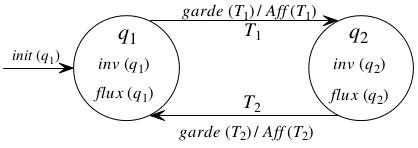
\includegraphics{images/automateHybride.jpeg}
	\caption{Automate hybride}
	\label{exempleAutomateHybride}
\end{figure}

L'\textit{état continu} du système est modélisé par un vecteur d'état continu $x(.)$ représentant un point dans un espace $X \subset \mathbb{R}^n$. Dans chaque sommet, la dynamique continue est modélisée par des conditions de flux telle que des équations différentielles ou des espaces d'états.

A chaque transition on associe un prédicat qui concerne l'état interne du système appelé \textit{garde}. Ce prédicat détermine les dates possibles pour le franchissement de la transition. Ainsi, une transition de l'automate hybride peut être franchie à l'instant $t$ si et seulement si sa garde est vérifiée par la valeur des variables d'état continues du système à l'instant considéré.

En général la garde d'une transition est exprimée par une région de l'espace d'état continu, qui peut se ramener à des intervalles.

L'ensemble des variables d'état continues mises à jour lors du franchissement d'une transition est décrit par une affectation. Les initialisations spécifiées par l'affectation correspondent à des fonctions, calculant la nouvelle valeur de l'état à partir de sa valeur avant le franchissement.

\begin{definition}{Un automate hybride d'ordre n, tel que présenté sur la figure \ref{exempleAutomateHybride} est défini par :}\\
\[\mathbb{A} = (Q, X, flux, inv, garde, Aff, init)\]
tel que :
\label{def:autom-hybride}
\begin{itemize}
\item Q = {$q_1, q_2, \ldots, q_m$} est un ensemble fini des sommets du graphe représentant les états discrets du système modélisé;
\item $X \subset \mathbb{R}^n$ est l'espace d'état continu. L'état continu du système est caractérisé à tout instant par le vecteur x = $[x_1, x_2, \ldots, x_n]^T$ dans l'espace Euclidien $\mathbb{R}^n$;
\item $flux(q_i)$ est la fonction qui affecte à chaque sommet une représentation pour l'évolution continue. Durant le séjour dans un sommet $q_i$ de l'automate hybride, l'évolution des variables continues est exprimée généralement sous la forme d'une équation d'état flux($q_i$) : $\dot{x} = \phi (q_i)(t,x,u)$, où $x \in X \subset \mathbb{R}^n$, $u \in U \subset \mathbb{R}^p$ et $\phi : X \times U \rightarrow X$;
\item L'invariant $inv(q_i)$ est une fonction qui associe à chaque sommet $q_i \in Q$ une contrainte sur les variables d'état continues x(.). Le système peut séjourner dans un sommet tant que l'invariant du sommet est satisfait;
\item $garde(T_i)$ est une fonction qui associe une condition de franchissement à chaque transition $T_i \in E$. Cette condition est en général une fonction logique entre des prédicats, portant sur les variables $x \in X$ et/ou ses dérivées $\dot{x} \in X$. Une transition $T_i \in E$ ne peut être franchie que si la condition $garde(T_i)$ est vraie;
\item L'affectation $Aff(T_i)$ est une fonction qui associe à chaque transition $T_i \in E$ une relation qui permet de mettre à jour la valeur des variables d'état après l'exécution de la transition $T_i$.
\item $init$ est une fonction qui affecte un état initial $x_0 \in X$ au sommet initial $q_{in} \in Q$. La condition initiale $init(q_{in})$ est un prédicat sur X.
\end{itemize}



\end{definition}


%\textbf{INSERER EXEMPLE SIMPLE : THERMOSTAT}
%\section{Éléments de stabilité}
\subsection*{Introduction}
Le but de cette partie est d'apporter des éléments généraux mais nécessaires à la compréhension et à la réussite de mon travail de stage. Dans un premier temps quelques rappels seront effectués sur la modélisation d'un système linéaire par espace d'état, puis sur les notions d'équilibre et de stabilité de ces systèmes. Ensuite nous introduirons les notions de stabilité au sens de Lyapunov. Enfin nous ferons un point sur les inéquations linéaires matricielles (LMI en anglais), qui nous seront utiles pour Lyapunov. %Nous finirons par les outils d'analyse à notre disposition.

\subsection{Systèmes Linéaires}

\begin{definition} Modèle d'état\\
\label{defmodeleEtat}
Soit un système vérifiant les hypothèses de linéarité, sa représentation d'état est donnée par : 
\[\dot{X}(t) = A(t).X(t) + B(t).U(t)\]
\[Y(t) = C(t).X(t) + D(t).U(t)\]
$X(t) \in \mathbb{R}^{n}$ est le vecteur d'état;\\
$Y(t) \in \mathbb{R}^{r}$ est le vecteur de sortie;\\
$U(t) \in \mathbb{R}^{m}$ est le vecteur des entrées;\\
$A(t) \in \mathbb{R}^{n\times n}$ est la matrice dynamique;\\
$B(t) \in \mathbb{R}^{n\times m}$ est la matrice de commande;\\
$C(t) \in \mathbb{R}^{r\times n}$ est la matrice de mesure ou de sortie;\\
$D(t) \in \mathbb{R}^{r\times m}$ est la matrice de transmission directe,
\end{definition}
Dans le cas général, un tel système est appelé système Linéaire à Temps Variant (LTV). Dans les cas particuliers où A, B, C et D sont constantes, le système est dit Linéaire à Temps Invariant (LTI).
Dans la suite nous considérerons les systèmes LTI.

\subsubsection{Notions de stabilité}
Parler de la stabilité d'un système est un abus de langage, en réalité nous devons parler de la stabilité d'un point d'équilibre, de fonctionnement ou d'une trajectoire de ce système.

\begin{definition} État d'équilibre\\
	\label{defEtatEq}
Un point $X_e$ de la trajectoire d'état est un état d'équilibre (point d'équilibre) si $X(t_0) = X_e \Leftrightarrow X(t) = X_e, \forall t \geq t_0$ en l'absence de commande et de perturbations.\\
Pour une représentation d'état comme vu précédemment, les points d'équilibre sont les solutions de l'équation : 
\[\dot{X}(t) = 0_{n,1} \Leftrightarrow A.X(t) = 0_{n,1}\]
\end{definition}


\begin{theo}
	\label{theoAinversible}
Un système continu LTI d'équations $\dot{X}(t) = A.X(t)$ peut avoir\\
- Un point d'équilibre unique X = 0 si A est inversible\\
- Une infinité de points d'équilibre si A n'est pas inversible	
\end{theo}

La stabilité permet de caractériser les points d'équilibre du système, c'est à dire que, si à un instant $t_0$, l'état d'équilibre est perturbé, l'état reviendra-t-il à cet état d'équilibre (stabilité) ou divergera-t-il (instabilité) ? Les différents types de stabilité sont présentés ci-après.

\begin{definition} Stabilité interne\\
	\label{defInterne}
L'état d'équilibre $X_e$ est dit \textbf{stable} si
\[ \forall \epsilon > 0, \exists\alpha > 0 \emph{ tel que si } ||X(0) - X_e|| \leq \alpha \emph{ alors } ||X(t) - X_e|| \leq \epsilon \]	
Dans le cas contraire, $X_e$ est dit \textbf{instable}.
\end{definition}

\begin{definition} Stabilité asymptotique\\
	\label{defAsymp}
L'état d'équilibre $X_e$ est dit \textbf{asymptotiquement stable} si
\[ \exists\alpha > 0 \emph{ tel que si } ||X(0) - X_e|| \leq \alpha \emph{ alors } \lim\limits_{t \rightarrow +\infty} X(t) = X_e \]
\end{definition}

\begin{definition} Stabilité exponentielle\\
	\label{defExpo}
L'état d'équilibre $X_e$ est dit \textbf{exponentiellement stable} s'il existe $\alpha > 0$ et $\lambda > 0$ tels que 
\[ \forall t > 0, \exists B_r(X_e,r), \forall X_0 \in B_r, ||X(t) - X_e|| \leq \alpha||X(0) - X_e||e^{-\lambda t} \]
où $B_r$ est une boule fermée de $\mathbb{R}^n$
\end{definition}

\begin{rem}
	\label{remImplique}
Il est possible de montrer que :
\begin{center}
stabilité exponentielle $\Rightarrow$ stabilité asymptotique $\Rightarrow$ stabilité interne
\end{center}
\end{rem}

Pour finir sur les notions de stabilité d'un système LTI, nous allons regarder la caractérisation de la stabilité. Soit le point d'équilibre $X_e$ du système décrit par un modèle d'état comme présenté à la définition \ref{defmodeleEtat}, alors la caractérisation de la stabilité s'étudie à partir de la matrice A. A possède r valeurs propres distinctes $\lambda_1,\ldots,\lambda_r$. Et nous avons le théorème suivant : 
\begin{theo} Conditions sur les valeurs propres\\
$Re(\lambda_i) > 0$ si il existe $i \in 1,\ldots,r$, alors $X_e$ est \textbf{instable}\\
$Re(\lambda_i) \leq 0$ pour tout $i \in 1,\ldots,r$, alors :\\
\vspace{-1cm}
\begin{tabbing}
	\hspace{1cm}\=\kill
	\> $Re(\lambda_i) < 0$ pour tout $i \in 1,\ldots,r$, alors $X_e$ est \textbf{asymptotiquement stable};\\ 
	\> $Re(\lambda_i) = 0$ et A diagonalisable, alors $X_e$ est \textbf{stable};\\ 
	\> $Re(\lambda_i) = 0$ et A non-diagonalisable, alors $X_e$ est \textbf{instable}.
\end{tabbing} 
\end{theo}

\subsubsection{Méthode directe de Lyapunov pour l'étude de stabilité}
Considérons la stabilité du point d'équilibre 0 pour les systèmes étudiés, en effet d'un point de vue physique, la méthode de Lyapunov s'apparente à regarder l'évolution de la fonction d'énergie. Donc étudier le point d'équilibre 0 est équivalent à étudier à quel moment le système n'aura plus d'énergie. 

Pour tout point d'équilibre $x_e \neq 0$, on pose le changement de variable \^{x}(t) = x(t)-$x_e$ et l'étude de la stabilité est identique à celle pour $x_e = 0$.
\begin{definition} Fonction candidate de Lyapunov\\
	\label{defFctLyap}
Soit $V : \mathbb{R}^n \rightarrow \mathbb{R}_+$ une fonction telle que : 
\begin{itemize}
\item[i)] V est continûment différentiable en tous ces arguments
\item[ii)] V est définie positive
\item[iii)] Il existe a et b deux fonctions de $\mathbb{R}_+$ dans $\mathbb{R}_+$, continues, monotones, non décroissantes, telles que
\[a(0) = b(0) = 0\]
\[\forall x \in \mathbb{R}^n a(||x||) \leq V(x) \leq b(||x||)\]
alors V est une fonction candidate de Lyapunov.
\end{itemize}
\end{definition}

\begin{rem}
La définition implique que la fonction V définit des équipotentielles imbriquées. C'est à dire que les courbes V(x) = cste, appelées \textbf{équipotentielles de Lyapunov}, définissent des domaines connexes autour de l'origine.
\end{rem}

\begin{theo} Stabilité locale\\
Si il existe une fonction $V$ dont les dérivées partielles premières sont continues et telle que :
\begin{itemize}
\item[1-] V est une fonction candidate de Lyapunov (Cf. définition \ref{defFctLyap})
\item[2-] $\dot{V}$ est localement semi-définie négative dans un voisinage de l'origine $\Omega$.
\end{itemize}

Alors le point d'équilibre 0 est \textbf{stable} et un domaine de conditions initiales stables est délimité par n'importe quelle équipotentielle de Lyapunov contenue dans $\Omega$.\\
Si $\dot{V}$ est localement définie négative dans $\Omega$, alors la stabilité est dite \textbf{localement asymptotique} dans la partie de l'espace délimitée par n'importe quelle équipotentielle de Lyapunov contenue dans $\Omega$.
\end{theo}

\begin{theo} Stabilité globale asymptotique\\
	\label{theoStabLyap}
S'il existe une fonction V telle que
\begin{itemize}
\item[1-] V est une fonction candidate de Lyapunov
\item[2-] $\dot{V}$ est définie négative
\item[3-] La condition $||x|| \rightarrow +\infty$ implique $V(x) \rightarrow +\infty$
\end{itemize}
alors 0 est un point d'équilibre globalement asymptotiquement stable.
\end{theo}

Le problème de cette méthode de Lyapunov est de trouver une fonction de Lyapunov pour le système considéré, en effet dans le cas non-linéaire il n'existe pas de méthode systématique. Dans le cas des systèmes LTI, il existe forcément une fonction de Lyapunov, mais elle n'est pas évidente à trouver.

\subsubsection{Application aux systèmes linéaires}
Dans ce cas, la représentation du système est donc classique : $\dot{x} = Ax$. Le point d'équilibre candidat est nécessairement $x = 0$. En choisissant $V(x) = x^TPx$ avec $P$ symétrique et définie positive ($P = P^T > 0$), la condition de stabilité asymptotique (Cf. Théorème \ref{theoStabLyap}) s'écrit alors 
\begin{center}
	$   \left \{
	\begin{array}{c c l}
	V(x) = x^TPx & > & 0, \forall x \\
	\dot{V}(x) = x^T(A^TP + PA)x & < & 0, \forall x
	\end{array}
	\right. $
\end{center}

\begin{theo}
Le système $\dot{x} = Ax$ est stable si et seulement si il existe une matrice définie positive P vérifiant le système LMI suivant : 
\begin{center}
$   \left \{
\begin{array}{r c l}
P & > & 0 \\
A^TP + PA & < & 0
\end{array}
\right. $
\end{center}
\end{theo}

\begin{theo}
	Dans le cas d'un système discret du type $x_{k+1} = Ax_k$, le théorème de stabilité devient (Lemme de Schur) :
	\begin{center}
		$   \left \{
		\begin{array}{r c l}
		P & > & 0 \\
		A^TPA - P & < & 0
		\end{array}
		\right. $
	\end{center}
	\label{theo:lyapDiscret}
\end{theo}

Par la suite nous travaillerons avec des systèmes LTI discret soumis à une commande, d'après les travaux de \cite{zhai_analysis_2007}, les conditions LMI deviennent : 
\begin{theo}
	Dans le cas d'un système discret du type $   \left \{
	\begin{array}{l}
	x_{k+1} = Ax_k + Bu_k \\
	y_k = Cx_k + Du_k
	\end{array}
	\right. $ :
	\begin{center}		
		$   \left \{
		\begin{array}{c c l}
		P & > & 0 \\
		\begin{bmatrix}
		A^TPA-P+C^TC	& A^TPB + C^TD \\ 
		B^TPA + D^TC	& B^TPB - I + D^TD  
		\end{bmatrix} & < & 0
		\end{array}
		\right. $
	\end{center}
	\label{theo:lyapDiscretAvecEntree}
\end{theo}
\subsubsection{Résumé pour l'étude de la stabilité}
\begin{itemize}
\item[1-] Trouver les points d'équilibre du système en résolvant Ax = 0
\item[2-] Linéariser le système autour des points d'équilibre pour évaluer la stabilité/instabilité des points d'équilibre (cette étape est souvent appelée première méthode de Lyapunov). Au voisinage d'un point d'équilibre $x_e$ :
\[\dot{x} = f(x) = A(x-x_e) + o(x-x_e)\]
Si la matrice A est définie négative, le système est localement asymptotiquement stable autour de $x_e$, mais aucun domaine de conditions initiales stables ne peut-être déterminé à ce stade.
Si A est semi-définie négative, on ne peut pas conclure. Sinon le point d'équilibre est instable.
\item[3-] Choisir une fonction candidate de Lyapunov V et, en posant le changement de variable \^{x} = x - $x_e$, étudier les domaines de stabilité/instabilité à l'aide de la seconde méthode de Lyapunov.
\item[4-] Si les résultats ne sont pas concluants, choisir une autre fonction de Lyapunov et recommencer.
\end{itemize}

%\subsubsection{Utilisation de MatLab pour l'étude de la stabilité (Lyapunov + LMI)}
%Cf. LyapunovLin.m pour un exemple de vérification de la seconde méthode de Lyapunov. Et voir switch\_test2.m pour avoir un exemple de projection des ellipses dans les différents plans de l'espace.
%
%\subsection{Éléments divers}
%Cette section va nous permettre de présenter différents points qui pourront être intéressants par la suite
%
%\subsubsection{D-stable}
%Une Matrice carré réelle A est dite (Hurwitz) D-stable si pour toute matrice diagonale positive D, la matrice DA est (Hurwitz) stable (à valeur propre strictement négative).
%
%Une matrice A est dites Hurwitz diagonalement stable si il existe une matrice positive P diagonale tel que A'P+PA est définie négative.
%
%A est Schur diagonalement stable si il existe une matrice positive P diagonale tel que A'PA-P est définie négative.
%
%Hurwitz diagonale stabilité est une condition suffisante pour la D-stabilité, mais l'inverse n'est vrai que pour une certaine classe de matrice. (Cf. On discrete-time diagonal and D-stability)


%\end{document}

%\section{La planification}
\subsection*{Introduction}
Le but de cette note est d'établir un état de l'art sur notre problème de planification de mission pour un drone. Nous cherchons à développer une méthode permettant la génération d'un plan faisable par le drone, c'est à dire que l'engin ne doit pas se retrouver dans une situation d'instabilité.

\subsection{Les différentes méthodes de planification}

\subsection{La planification appliquée aux mission de drone}
\cite{CHA05} présente une architecture très intéressante pour le problème de planification de mission pour un drone : 
\begin{itemize}
	\item niveau 3 : gestion de la mission et de son environnement, ce niveau permet de prendre en compte une modification de l'environnement de mission du drone, et donc de demander un nouveau plan (niveau 2)
	\item niveau 2 : Gestion du plan, ce niveau permet le calcul effectif d'un plan (demandé par le niveau 3, ou le niveau 1 si un segment du plan n'est pas conforme)
	\item niveau 1 : Gestion de la trajectoire, ce niveau permet le calcul d'une trajectoire pour le segment de plan donné par le niveau 2, il doit ressortir l'ensemble des points que doit suivre le drone pour réaliser ce segment du plan, si le niveau 0 considère que le prochain point n'est pas atteignable, le niveau 1 doit calculer une nouvelle trajectoire pour ce même segment
	\item 0 : guidage, ce niveau permet le guidage du drone, il doit informer le niveau 1 si le prochain point est atteignable ou pas, si il l'est, il demande à la couche de commande d'effectuer les actions nécessaires pour aller à ce point (modification de l'angle d'incidence, augmentation de la poussée etc...
\end{itemize}
Dans ce travail, les niveaux 3 et 2 ont était traité, les niveaux inférieurs ont était considéré comme connu. Le niveau 1 peut être vu comme du motion planning (un drone est vu comme un robot non-holonome), le niveau 0 lui peut être vu comme la boucle de commande du drone (modélisation continu, contraintes LMIs pour la stabilité), mais cette commande doit intégrer des aspects discret (mission) et continu (mécanique du vol, stabilité), nous pouvons donc émettre l'hypothèse qu'un modèle hybride serait utile.

Dans le monde de la robotique il existe une sous branche du motion planning : Kinodynamic planning, c'est à dire que l'on va prendre en compte (dès la phase de planification) la dynamique du robot (contrainte non-holonome, stabilité ...)
Alors qu'avec l'architecture proposée dans \cite{cha05}, le niveau 2 donne un plan non contraint par la dynamique, le niveau 1 donne une trajectoire elle aussi non contrainte par la dynamique, et c'est seulement le niveau 0 qui est capable de faire remonter des informations sur l'aspect réalisable du mouvement ou pas.

%\subsection{Thèse DICHEVA 2012}
\cite{DIC12} Ce travail de thèse porte une attention soutenue à la planification de mission pour le drone Eole. Il permet d'avoir un état de l'art récent sur les aspects de planification pour drone, ainsi que pour les architectures de mission.

L'architecture proposée est globalement la même que celle de CHANTERY vue ci-dessus, mais dans ce travail tout les niveaux ont était traité (Cf. page 180) : 
\begin{itemize}
	\item niveau 2 : Planification de mission : Un algorithme A* en 3D est proposé (avec une extension "4D" pour intégrer le temps). Cette planification peut-être apparenté à la KinoDynamic planning car l'auteur prends en compte dans ce niveau du rayon minimal de virage ainsi que la pente maximale.
	\item niveau 1 : Génération de trajectoire : Cette partie est solutionnée par l'utilisation de polynômes cartésiens d'ordre 3
	\item niveau 0 : Suivi de trajectoire : Cette étape est réalisée en utilisant une commande par mode glissant.
	\item niveau 0 bis : Modélisation de l'aéronef
\end{itemize} 

Le chapitre 5 de ce travail détaille le niveau 0 (suivi de trajectoire), car il est lui même décomposé de 4 éléments distincts.

Dans ce travail l'algorithme de planification est très intéressant car il permet la prise en compte d'un plan 3D, la modélisation de Eole est assez détaillée, de plus la prise en compte d'un modèle météo a été effectuée.

Mais ce travail, même s'il résout le problème de planification pour un drone, suppose que les restrictions faites au niveau 2 (KinoDynamic) sont suffisante pour assurer la stabilité du drone sur l'ensemble du plan.



%%\phantomsection\addcontentsline{toc}{section}{Références}
\begin{thebibliography}{ABC}	
    \bibitem{kur02} Monika KUROVSKY. \emph{Etude des systèmes dynamiques hybrides par représentation d'état discrète et automate hybride.}. Institut National Polytechnique Grenoble - INPG, 2002.
    \bibitem{cha05} Elodie CHANTERY. \emph{Planification de mission pour un véhicule aérien autonome}. École nationale supérieure de l'aéronautique et de l'espace, 2005.
    \bibitem{art06} Christian ARTIGUES, Dominique FEILLET. \emph{Une méthode exacte pour le problème d'ordonnancement d'atelier avec temps de préparation}. Écoles des Mines d'Alès, 2006.
    \bibitem{her07} Florent HERNANDEZ. \emph{Model-chechking et ordonnancement : Application à la décision de protection phytosanitaire de la vigne}. CEMAGREF, 2007.
    \bibitem{yalmip} Johan LÖFBERG. \emph{A toolbox for modeling and optimization in MATLAB}. Automatic Control Laboratory, 2004.
    \bibitem{goe09} Goebel, R. ; Sanfelice, R.G. et Teel, A. \emph{Hybrid dynamical systems : Robust stability and control for systems that combine continuous-time and discrete-time dynamics}. IEEE Control Systems, 2009.
    \bibitem{boy94} S. BOYD, L. El GHAOUI, E. FERON, V. BALAKRISHNAN. \emph{Linear matrix inequalities in system and control theory}. SIAM, 1994.
	\bibitem{arz08} Denis ARZELIER. \emph{Course on LMI optimization with applications in control : part II.1 and II.2}. LAAS, 2008.
	\bibitem{dic12} Svetlana DICHEVA. \emph{Planification de mission pour un système de lancement aéroporté autonome}. Université d’Evry-Val d’Essonne, 2012.
\end{thebibliography}



%\end{document}


\chapter{Modélisation}
\label{chapter:model}
Dans ce chapitre nous allons détailler la modélisation que nous avons mis en place d'un point de vue général. Le chapitre suivant présentera différents solveurs CSP que nous avons testé ainsi que l'application de cette modélisation dans ces solveurs. Nous verrons que la facilité de représentation des contraintes diffère grandement selon les solveurs utilisés.
\section{Le formalisme de planification}
Afin d'avoir plus de flexibilité de représentation, et notamment pour pouvoir prendre en compte des calculs mathématiques dans notre problème de planification, nous avons souhaité ne pas passer par une représentation STRIPS ou PDDL du problème. Nous souhaitons pouvoir uniquement utiliser une représentation CSP. Cela va nous permettre d'intégrer des contraintes mathématiques, ainsi que des contraintes quadratiques à notre problème de planification.

L'idée est de définir un nombre $k$ d'état du problème, $k$ est appelé l'horizon du problème. Ensuite nous devons traduire les actions possibles, celles-ci ont des pré-conditions définies par des contraintes sur des états à l'instant $k$, et des effets définis par des contraintes sur des états à l'instant $k$ et/ou $k+1$.

\begin{definition} Un problème de planification utilisant le formalisme des CSP peut donc être défini comme un 5-uplet $(\mathcal{S},\mathcal{D},\mathcal{C},\mathcal{I},\mathcal{G})$ où:
	\label{def:CSP-planif}
	\begin{itemize}
		\item $\mathcal{S} = \{S_{11}, \dots, S_{1n}, \dots, S_{k1}, \dots, S_{kn}\}$ est l'ensemble des variables du problème, avec $n$ le nombre de variable à chaque instant;
		\item $\mathcal{D} = \{\mathcal{D}_1, \dots, \mathcal{D}_n \}$ est l'ensemble des domaines des variables;
		\item $\mathcal{C} = \{C_1, \dots, C_m \}$ est un ensemble de contraintes;
		\item $\mathcal{I} \in \mathcal{C}$ est l'ensemble des contraintes définissant l'état initial du problème;
		\item $\mathcal{G} \in \mathcal{C}$ est l'ensemble des contraintes définissant les buts du problème. 
	\end{itemize}
\end{definition}

\begin{definition} Les états du problème sont définis tels que $\mathcal{E} = \{E_1, \dots, E_k\}$, avec $E_k = \{S_{k1}, \dots, S_{kn}\}$. 
	\label{def:etat-csp-planif}
\end{definition}

Dans un problème de planification nous pouvons distinguer différents types de contraintes \cite{artificial_15} parmi lesquels : 
\begin{itemize}
	\item Les \textbf{contraintes d'état} permettent d'imposer des relations entre des variables à l'instant $k$;
	\item Les \textbf{contraintes de pré-condition} entre des variables à l'instant $k$, celles-ci permettent de définir quelles actions sont disponibles dans cet état;
	\item Les \textbf{contraintes d'effets} qui en fonction des actions disponibles à l'instant $k$, contraignent la valeur de certaines variables à l'instant $k+1$;
	\item Les \textbf{contraintes d'actions}, qui spécifient quelles actions ne peuvent pas être actives simultanément (contraintes mutex);
	\item Les \textbf{contraintes d'état initial} $\mathcal{I}$ sur des variables à l'instant $k=0$;
	\item Les \textbf{contraintes de but} $\mathcal{G}$ permettant de donner un objectif à la planification, les objectifs peuvent survenir à des instants quelconques.
\end{itemize}

\section[Modélisation et analyse]{Modélisation et analyse de stabilité de l'aéronef}
Pour rappel, nous cherchons à déterminer une méthode permettant de savoir si un aéronef est capable d'effectuer une mission donnée (objectif, environnement...), tout en s'assurant que l'engin reste stable.
Afin de restreindre le cadre de travail autour de l'aéronef, nous avons émis quelques hypothèses :
\begin{itemize}
\item Le modèle utilisé par la suite doit être \textbf{linéaire};
\item Le modèle de l'aéronef doit intégrer le modèle \textbf{aérodynamique} de l'avion ainsi que la boucle de \textbf{contrôle};
\item L'évolution du système, donc les changements de loi de pilotage, sont représentées par un \textbf{automate hybride} autonome (Déf. \ref*{def:autom-hybride}).
\end{itemize}

\subsection{Encodage d'un espace d'état}
Un système représenté par un espace d'état à l'instant $k$ est caractérisé par 4 matrices $A, B, C, D$, par un vecteur d'entrée $U_k$, par un vecteur de sortie $Y_k$, par un vecteur $X_k$ représentant l'état présent et par un vecteur $X_{k+1}$ représentant l'état suivant :
\begin{equation}
   \left \{
\begin{array}{l}
X_{k+1} = A.X_k + B.U_k \\
Y_k = C.X_k + D.U_k
\end{array}
\right. 
\label{eq:espaceEtat}
\end{equation}
De manière générale, un solveur CSP n'est pas capable de gérer les produits matriciels, c'est pourquoi nous les traduirons par des opérateurs plus simples tels que des sommes de produits : 
\begin{equation}
\left \{
\begin{array}{l}
\forall k, \forall i \in \{1 \ldots n\}, X_{k+1}(i) = \sum_{j=1}^{n} A(i,j)\times X_k(j) + \sum_{j=1}^{m} B(i,j)\times U_k(j) \\
\forall k, \forall i \in \{1 \ldots r\}, Y_k(i) = \sum_{j=1}^{n} C(i,j)\times X_k(j) + \sum_{j=1}^{m} D(i,j)\times U_k(j)
\end{array}
\right. 
\label{eq:espaceEtatExplose}
\end{equation}

\subsection{Encodage de l'automate hybride autonome}
Nous considérons dans ces travaux que les changements de mode - de loi - de pilotage sont autonomes. Le changement de mode est donc une conséquence de la commande appliquée au système, or nous souhaitons justement planifier la commande à appliquer afin de suivre une mission. Le planificateur doit donc être capable de prendre en compte ces changements de mode lorsqu'il calcule l'état suivant du système.

Nos changements de loi de pilotage sont modélisés par un automate hybride (Cf. Déf \ref{def:autom-hybride}). Pour traduire les aspects hybrides, nous décomposons les dynamiques en deux : 
\begin{itemize}
	\item Fonction de transition discrète :
	\[\mathcal{F}_d : \mathbb{R}^{n+m}\times \mathit{E}_p \rightarrow \mathit{E}_s\]
	Permet de déterminer le mode de fonctionnement suivant en fonction des entrées, de l'état et du mode actuel.
	\item Fonction de transition continue : 
	\[\mathcal{F}_c : \mathbb{R}^{n+m}\times \mathit{E}_p \times \mathit{E}_s \rightarrow \mathbb{R}^{n+r}\]
	Permet de calculer l'état suivant et les sorties du systèmes en fonction de l'état actuel, des entrées, des modes de fonctionnement présent et suivant.
\end{itemize}
%Avec $\mathit{E}_p$ et $\mathit{E}_s$ l'ensemble des états présents et suivants.

%Pour ce faire nous nous sommes appuyé sur une démarche classique de mise en œuvre des systèmes à événements discrets : à chaque instant, nous regardons les conditions de sortie  

%\subsection{Les contraintes de stabilité}
%\label{subsection:contrainteStabilite}
%Afin d'étudier la stabilité de nos lois de commande, nous avons choisi d'utiliser le formalisme et la méthode de Lyapunov décrite dans le théorème \ref{theoStabLyap}. Notre démarche pour garantir la stabilité du système global est la suivante : 
%\begin{itemize}
%	\item Pour chaque mode de fonctionnement nous déterminons la matrice $P_i$ (liée au i-ème mode) respectant les contraintes LMI présentée dans le théorème \ref{theo:lyapDiscretAvecEntree};
%	\item Une fois que nous avons les $P_i$ nous considérons les ellipsoïdes de taille n : $\mathcal{E}_i = x^TP_ix < 1$ (\cite{gains_ufr_2001} Cf. 1.6.2.3). Ces ellipsoïdes garantissent la stabilité pour tout point de départ du système qui se situe à l'intérieur de l'ellipsoïde, en dehors on ne peut pas conclure;
%	\item Pour finir nous venons rajouter ces contraintes ellipsoïdales aux conditions de l'automate hybride. En effet, à un instant donné nous avons un état $x_k$ pour notre système, si le système doit passer du mode i au mode j, alors $x_k$ doit satisfaire les conditions $\mathcal{E}_i$ et $\mathcal{E}_j$.
%\end{itemize}

%\pagebreak
\subsection{Les contraintes de stabilité}
\label{subsection:contrainteStabilite}
Afin d'étudier la stabilité de notre système, nous avons choisi d'utiliser le formalisme et la méthode de Lyapunov décrite dans la partie \ref{subsubsec:applicationStabHybride}. Notre démarche pour garantir la stabilité du système global est la suivante : 
\begin{itemize}
	\item Pour chaque mode de fonctionnement nous déterminons la matrice $P_i$ (liée au i-ème mode) respectant les contraintes LMI présentées dans le théorème \ref{theo:lyapDiscretHybride};
	\item Une fois que nous avons les $P_i$ nous considérons les fonctions d'énergie : $V_i(x) = x^TP_ix$;
	\item Pour finir nous venons rajouter ces contraintes aux conditions de l'automate hybride. En effet, à un instant donné nous avons un état $x_k$ pour notre système, si le système doit passer du mode i au mode j, alors nous devons vérifier que la fonction d'énergie globale décroisse : $V_j(x_{k+1})-V_i(x_k) \leq 0$
\end{itemize}
Un exemple d'évolution de la fonction d'énergie que nous souhaitons garantir est donnée sur la figure \ref{fig:decroissance} :
%\vspace{-12cm}
\begin{figure}[h]
	\centering	
	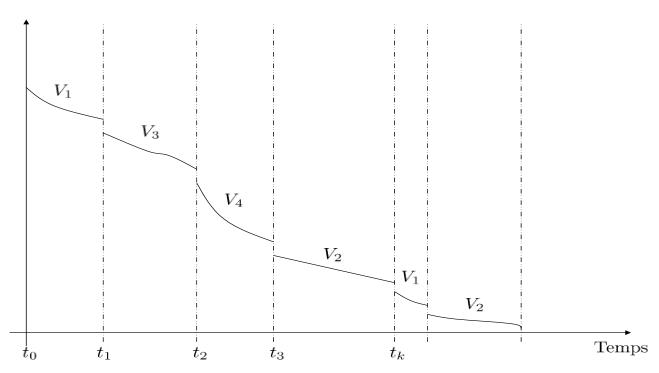
\includegraphics[scale=0.4]{images/decroissance.png}
	\caption{Évolution de la fonction d'énergie par morceaux}
	\label{fig:decroissance}
\end{figure}
%\pagebreak
\section{Le cas d'étude}
A présent, nous allons voir comment modéliser une mission de planification sur un cas concret, donc en intégrant le modèle d'un aéronef. Pour cela nous commencerons par présenter l'environnement et le modèle de l'aéronef. Ensuite nous décrirons les variables de notre problème, puis les contraintes.
\subsection{Le monde et l'aéronef}
La figure \ref{fig:scenarioVierge2} représente le monde et la mission (zones à éviter, point de départ et arrivée).
\begin{figure}[h]
	\centering	
	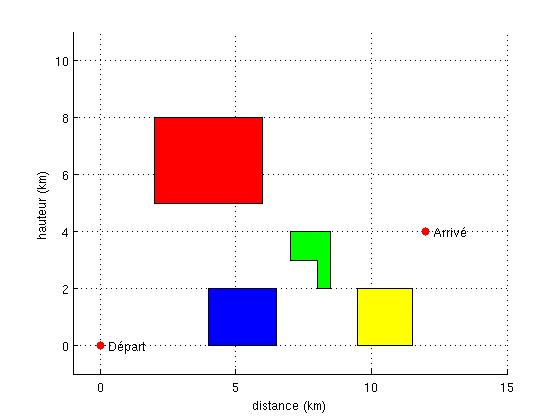
\includegraphics[scale=0.42]{images/scenarioVierge2.jpg}
	\caption{Environnement d'une mission}
	\label{fig:scenarioVierge2}
\end{figure}

L'aéronef que nous considérons pour cet exemple est celui sur lequel nous avons fait les tests lors de ce stage. Nous sommes partis d'un modèle non-linéaire (sous simulink) d'un avion de ligne présentant des changements de lois de pilotage autonome, et nous en avons extrait trois modèles linéaires (sous forme d'espace d'état Déf. \ref{defmodeleEtat}) représentant chaque mode de fonctionnement de façon séparée. Il est à noter que nous travaillons uniquement dans le plan longitudinal, donc la dynamique latérale n'est pas représentée dans ce modèle.
L'automate hybride résultant de cette manipulation est présenté sur la figure \ref{fig:modeleHybride}.
\begin{figure}[h]		
	\centering	
	\scalebox{0.8}{%
		\begin{tikzpicture}[->,>=stealth',shorten >=0pt,auto,node distance=0cm,
		semithick,every text node part/.style={align=center}]
		\tikzstyle{every state}=[fill=white,draw=black,text=black]

		%\node   (A)   at (2,1)  {};
		\node[state]    (maintien)  at (3,1.5)     {Maintien\\$-\epsilon < switch < \epsilon $};
		%\draw[<-] (B) to[bend right] (A)  ;
		
		\node[state]    (monter)   at (-2,-3.5)     {Montée\\$switch \geq \epsilon$ };
		\node[state]    (descendre)   at (8,-3.5)     {Descente\\$switch \leq -\epsilon$};
		
		\path 
		(maintien) edge [bend left=10]		node[below]{$switch \leq -\epsilon$}   (monter)		
		(maintien) edge [bend right=10] 	node[below]{$switch \geq \epsilon$}   (descendre)
		
		(monter) edge [bend left=10] 	node[left]{$switch < \epsilon$}   (maintien)		
		(monter) edge [bend left=10] 	node[above]{$switch \leq -\epsilon$}   (descendre)	
		
		(descendre) edge [bend left=10] 	node[below]{$switch \geq \epsilon$}  (monter)	
		(descendre) edge [bend right=10] 	node[right]{$switch > -\epsilon$}  (maintien)
		
		(maintien) edge [loop above]    	node[anchor=north,above]{} (maintien)	
		(monter) edge [loop below]    	node[anchor=south,below]{} (monter)
		(descendre) edge [loop below]    	node[anchor=south,below]{} (descendre);
		
		\end{tikzpicture} }
	\caption{Automate hybride autonome avec 3 lois de pilotage}
	\label{fig:modeleHybride}
\end{figure}

A chaque instant l'avion peut être dans un seul mode de fonctionnement, les changements de mode sont autonomes et se font en fonction de la valeur de $switch = |H_c - H|$, c'est à dire en fonction de la différence entre l'altitude de consigne et l'altitude réelle de l'avion.
Cette condition de switch et la valeur du $\epsilon$ sont imposées par le systèmes de l'avion.

A présent nous souhaitons savoir si cet aéronef est capable de remplir la mission donnée dans le monde décrit ci-dessus. La suite de ce chapitre va donc expliquer comment traduire cet exemple sous la forme d'un planificateur en CSP comme présenté dans la définition \ref{def:CSP-planif}.

\subsection{Les variables}
\label{subSec:variables}
Nous choisissons de distinguer trois différentes types de variables, les variables de \textbf{définition}, considérées comme constantes pour le planificateur. Les variables de \textbf{décision}, ce sont les variables sur lesquelles le planificateur a de la liberté. Enfin les variables de \textbf{fonction}, le planificateur ne peut pas directement fixer la valeur de ces variables, elles dépendent de variables de décision et de variable de définition. Cette distinction se retrouve dans certains outils de satisfaction de contraintes ou d'optimisation sous contraintes.
\pagebreak
\subsubsection{Les variables de définition}
\begin{itemize}		
	\item Les bornes du monde :
		\subitem $H_{max} \in \mathbb{R}^+$ : altitude maximale;
		\subitem $L_{max} \in \mathbb{R}^+$ : Longueur maximale; 
		\subitem $H_{min} \in \mathbb{R}^+$ : altitude minimale;
		\subitem $L_{min} \in \mathbb{R}^+$ : Longueur minimale; 
	\item Le point de départ :
		\subitem $H_{init} \in \mathbb{R}^+$ : altitude initiale;
		\subitem $L_{init} \in \mathbb{R}^+$ : distance initiale;
	\item Le point d'arrivé :
		\subitem $H_{goal} \in \mathbb{R}^+$ : altitude objectif;
		\subitem $L_{Goal} \in \mathbb{R}^+$ : distance objectif;
	\item L'aéronef :
		\subitem $Va_{min} \in \mathbb{R}^+$ : vitesse minimale;		\subitem $Va_{max} \in \mathbb{R}^+$ : vitesse maximale;
		\subitem $\alpha_{min} \in \mathbb{R}$ : angle d'incidence minimal;		\subitem $\alpha_{max} \in \mathbb{R}$ : angle d'incidence maximal;
	\item Autres :
	\subitem $step \in \mathbb{N}$ : le nombre d'itération, permet d'imposer au planificateur de tenter de résoudre le problème en un nombre d'itération fixé (lié au pas de temps);
	\subitem $t_{init} \in \mathbb{R}$ : l'instant initial du problème (en général $t(0) = 0$);
	\subitem $T_s \in \mathbb{R}^+$ : le pas de temps du système;
	\subitem $\epsilon \in \mathbb{R}^+$ : permet de définir la précision de l'objectif.
\end{itemize}	

\subsubsection{Les variables de décision}
\label{variableDecision}
Dans notre cas, nous souhaitons planifier la commande à appliquer à notre avion, cela revient à déterminer les valeurs du vecteur $U_k$ (Cf. éq \ref{eq:espaceEtat}). 

%Nous rappelons que notre planificateur doit travailler sur un horizon de temps borné à un nombre d'itération fixé. Chaque variable doit donc être calculée (et stockée) à chaque instant $k \in \{0, \ldots, step-1\}$.

Nous rappelons que notre planificateur doit travailler sur un horizon de temps borné à un nombre d'itérations fixé. Chaque variable doit donc être calculée (et stockée) à chaque instant $k \in \mathbb{N}^{step}$.

De plus, sur cet exemple nous n'avons que deux entrées :
\begin{itemize}	
	\item $\forall k, Vac_{k} \in \{Va_{min}, \ldots, Va_{max}\}$ : vitesse horizontale de consigne;	
	\item $\forall k, Hc_{k} \in \{H_{min}, \ldots, H_{max}\}$ : l'altitude de consigne.	
\end{itemize}

\subsubsection{Les variables de fonction}
\label{variableFonction}
Ce sont les variables les plus compliquées à définir, ce sont en général des fonctions mathématiques prenant en entrée plusieurs autres variables.

\underline{Les états du système} conditionnés par le mode de fonctionnement actuel ({$\mathbf{X_{k+1}}$}) :\\
\[\forall k, (mode_k == -1) \Rightarrow X_{k+1}(i) = \sum_{j=0}^{n-1} A_{descente}(i,j)\times X_k(j) + \sum_{j=0}^{m-1} B_{descente}(i,j)\times U_k(j)\]
\[\forall k, (mode_k == 0) \Rightarrow X_{k+1}(i) = \sum_{j=0}^{n-1} A_{maintien}(i,j)\times X_k(j) + \sum_{j=0}^{m-1} B_{maintien}(i,j)\times U_k(j)\]
\[\forall k, (mode_k == 1) \Rightarrow X_{k+1}(i) = \sum_{j=0}^{n-1} A_{mont\acute{e}}(i,j)\times X_k(j) + \sum_{j=0}^{m-1} B_{mont\acute{e}}(i,j)\times U_k(j)\]

\underline{Les 3 sorties du système} conditionnées par le mode de fonctionnement actuel ($\mathbf{Va_k, H_k}$ et $\mathbf{\alpha_k}$):\\
\[\forall k, (mode_k == -1) \Rightarrow 
	\left \{
	\begin{array}{l}
	Va_k = \sum_{j=0}^{n-1} C_{descente}(0,j)\times X_k(j) + \sum_{j=0}^{m-1} D_{descente}(0,j)\times U_k(j) \\
	H_k = \sum_{j=0}^{n-1} C_{descente}(1,j)\times X_k(j) + \sum_{j=0}^{m-1} D_{descente}(1,j)\times U_k(j) \\
	\alpha_k = \sum_{j=0}^{n-1} C_{descente}(2,j)\times X_k(j) + \sum_{j=0}^{m-1} D_{descente}(2,j)\times U_k(j)
	\end{array}
	\right.\]
	
	\[\forall k, (mode_k == 0) \Rightarrow 
	\left \{
	\begin{array}{l}
	Va_k = \sum_{j=0}^{n-1} C_{maintien}(0,j)\times X_k(j) + \sum_{j=0}^{m-1} D_{maintien}(0,j)\times U_k(j) \\
	H_k = \sum_{j=0}^{n-1} C_{maintien}(1,j)\times X_k(j) + \sum_{j=0}^{m-1} D_{maintien}(1,j)\times U_k(j) \\
	\alpha_k = \sum_{j=0}^{n-1} C_{maintien}(2,j)\times X_k(j) + \sum_{j=0}^{m-1} D_{maintien}(2,j)\times U_k(j)
	\end{array}
	\right.\]
	
	\[\forall k, (mode_k == 1) \Rightarrow 
	\left \{
	\begin{array}{l}
	Va_k = \sum_{j=0}^{n-1} C_{mont\acute{e}}(0,j)\times X_k(j) + \sum_{j=0}^{m-1} D_{mont\acute{e}}(0,j)\times U_k(j) \\
	H_k = \sum_{j=0}^{n-1} C_{mont\acute{e}}(1,j)\times X_k(j) + \sum_{j=0}^{m-1} D_{mont\acute{e}}(1,j)\times U_k(j) \\
	\alpha_k = \sum_{j=0}^{n-1} C_{mont\acute{e}}(2,j)\times X_k(j) + \sum_{j=0}^{m-1} D_{mont\acute{e}}(2,j)\times U_k(j)
	\end{array}
	\right.\]	
	
	\underline{Initialisation du mode} ($\mathbf{mode_0}$) :\\
	$(H_{goal} - H_{init}) \geq \epsilon \Rightarrow mode_0 = 1$ \\
	$(H_{goal} - H_{init}) \leq -\epsilon \Rightarrow mode_0 = -1$ \\
	$(\rceil((H_{goal} - H_{init}) \geq \epsilon) \wedge \rceil((H_{goal} - H_{init}) \leq -\epsilon) \geq \epsilon) \Rightarrow mode_0 = 0$ 
			
	\underline{La condition de switch} de l'automate hybride ($\mathbf{switch_k}$) :\\
	$\forall k, switch_k = Hc_k - H_k$
	
	\underline{La dynamique discrète} de l'automate ($\mathbf{mode_{k+1}}$):\\
	$\forall k < step, (mode_k == -1) \wedge (switch_k \geq \epsilon) \Rightarrow mode_{k+1} = 1$\\
	$\forall k < step, (mode_k == -1) \wedge (switch_k > -\epsilon) \Rightarrow mode_{k+1} = 0$ \\
	$\forall k < step, (mode_k == -1) \wedge (\rceil(switch_k \geq \epsilon) \wedge \rceil(switch_k > -\epsilon)) \Rightarrow mode_{k+1} = -1$\\ \\	
	$\forall k < step, (mode_k == 0) \wedge (switch_k \leq -\epsilon) \Rightarrow mode_{k+1} = 1$\\
	$\forall k < step, (mode_k == 0) \wedge (switch_k \geq \epsilon) \Rightarrow mode_{k+1} = -1$ \\
	$\forall k < step, (mode_k == 0) \wedge (\rceil(switch_k \leq -\epsilon) \wedge \rceil(switch_k \geq \epsilon)) \Rightarrow mode_{k+1} = 0$\\ \\	
	$\forall k < step, (mode_k == 1) \wedge (switch_k < \epsilon) \Rightarrow mode_{k+1} = 0$\\
	$\forall k < step, (mode_k == 1) \wedge (switch_k \leq -\epsilon) \Rightarrow mode_{k+1} = -1$ \\
	$\forall k < step, (mode_k == 1) \wedge (\rceil(switch_k < \epsilon) \wedge \rceil(switch_k \leq -\epsilon)) \Rightarrow mode_{k+1} = 1$
			
	\underline{Le temps} ($\mathbf{t_k}$) :\\
	$\forall k, t_k = t_{init} + T_s\times k$
	
	\underline{La distance parcourue} ($\mathbf{L_k}$) :\\
	$\forall k, L_k = L_{init} + Va_k\times T_s$
	
	\underline{La fonction de coût}, il s'agira ici de minimiser l'écart entre l'altitude objectif et l'altitude réelle au dernier instant de temps :\\
	$but = |H_{step-1} - H_{goal}|$
	


\subsection{Les contraintes}
A l'aide des variables décrites précédemment nous pouvons définir les contraintes CSP permettant au solveur de prendre en compte les obstacles, les bornes du monde etc...

	\underline{Le monde} : \\
	$\forall k, Va_{min} \leq Va_k \leq Va_{max}$ : contrainte sur la vitesse réelle.\\
	$\forall k, H_{min} \leq H_k \leq H_{max}$ : contrainte sur l'altitude réelle.\\
	$\forall k, \alpha_{min} \leq \alpha_k \leq \alpha_{max}$ : contrainte sur l'angle d'incidence réel.\\
	$\forall k, L_{min} \leq L_k \leq L_{max}$ : permet de connaitre la position en distance de l'avion.\\	
	\underline{Les obstacles} : \\
	Nous allons détailler ici les 4 zones présentées sur la figure \ref{fig:scenarioVierge2}. \\
	zone rouge : $\forall k, 2 \leq L_k \leq 6 \Rightarrow H_k > 8 \vee H_k < 5$\\
	zone bleue : $\forall k, 4 \leq L_k \leq 6.5 \Rightarrow H_k > 2$\\
	zone verte : $\forall k,   \left \{
	\begin{array}{l}
	7 \leq L_k < 8.5 \Rightarrow H_k > 4 \vee H_k < 3 \\
	8.5 \leq L_k \leq 9 \Rightarrow H_k > 4 \vee H_k < 2
	\end{array}
	\right.$\\
	zone jaune : $\forall k, 9.5 \leq L_k \leq 11.5 \Rightarrow H_k > 2$\\
	\underline{La mission} : \\
	$H_{0} == H_{init}$ : permet d'imposer l'altitude initiale.\\
	$L_{0} == L_{init}$ : permet d'imposer la distance initiale.\\
	$H_{goal} - \epsilon \leq H_{step} \leq H_{goal} + \epsilon$ : permet de définir une altitude à atteindre avec une incertitude de précision\\
	$l_{goal} - \epsilon \leq L_{step} \leq L_{goal} + \epsilon$ : permet de définir une distance à atteindre avec une incertitude de précision\\
	\underline{La stabilité} :\\
	Pour rappel, nous souhaitons que l'aéronef reste dans son domaine de stabilité à chaque instant, et ce, même lors d'un changement de mode. Pour cela nous reprenons les résultats présentés dans la partie \ref{subsubsec:stabHybride}, c'est à dire qu'à chaque changement de mode, la valeur de la fonction $V(x) = x^TPx$ doit diminuer.
	
	 %Pour cela nous proposons qu'à chaque instant, le système (donc le vecteur $x_k$) respecte les contraintes ellipsoïdales décrites dans le paragraphe \ref{subsection:contrainteStabilite}. De plus lors d'un changement de mode, nous souhaitons que $x_k$ soit dans l'intersection des ellipsoïdes des 2 modes en question.
	
	Pour faciliter l'écriture des contraintes, nous introduisons les notations suivantes : 
%	\vspace{-1cm}
	\begin{tabbing}
		\hspace{5cm}\=\hspace{5cm}\=\kill
	$\mathcal{V}_{-1,k} = x_k^TP_{descente}x_k$	\> $\mathcal{V}_{0,k} = x_k^TP_{maintien}x_k$ \> $\mathcal{V}_{1,k} = x_k^TP_{mont\acute{e}e}x_k$
	\end{tabbing} 
%	\begin{itemize}
%		\centering
%		\item[ ] $\mathcal{V}_{-1,k} = x_k^TP_{descente}x_k$;
%		\item[ ] $\mathcal{V}_{0,k} = x_k^TP_{maintien}x_k$;
%		\item[ ] $\mathcal{V}_{1,k} = x_k^TP_{mont\acute{e}e}x_k$;
%		%\item[ ] $\mathcal{E}_{-1,k}$ représente l'ellipsoïde du mode descente à l'instant k : $x_k^TP_{descente}x_k < 1$;
%		%\item[ ] $\mathcal{E}_{0,k} \equiv x_k^TP_{descente}x_k < 1$;		%\item[ ] $\mathcal{E}_{1,k} \equiv x_k^TP_{mont\acute{e}}x_k < 1$.
%	\end{itemize}
	
%	Les contraintes sont donc les suivantes :
%	$\forall k, (mode_k == 0) \wedge (mode_{k+1} == 0) => \mathcal{E}_{0,k} \wedge \mathcal{E}_{0,k+1}$\\
%	$\forall k, (mode_k == 0) \wedge (mode_{k+1} == -1) => \mathcal{E}_{0,k} \wedge \mathcal{E}_{-1,k} \wedge \mathcal{E}_{0,k+1} \wedge \mathcal{E}_{-1,k+1}$\\
%	$\forall k, (mode_k == 0) \wedge (mode_{k+1} == 1) => \mathcal{E}_{0,k} \wedge \mathcal{E}_{1,k} \wedge \mathcal{E}_{0,k+1} \wedge \mathcal{E}_{1,k+1}$\\\\
%	$\forall k, (mode_k == -1) \wedge (mode_{k+1} == -1) => \mathcal{E}_{-1,k} \wedge \mathcal{E}_{-1,k+1}$\\
%	$\forall k, (mode_k == -1) \wedge (mode_{k+1} == 0) => \mathcal{E}_{-1,k} \wedge \mathcal{E}_{0,k} \wedge \mathcal{E}_{-1,k+1} \wedge \mathcal{E}_{0,k+1}$\\
%	$\forall k, (mode_k == -1) \wedge (mode_{k+1} == 1) => \mathcal{E}_{-1,k} \wedge \mathcal{E}_{1,k} \wedge \mathcal{E}_{-1,k+1} \wedge \mathcal{E}_{1,k+1}$\\\\
%	$\forall k, (mode_k == 1) \wedge (mode_{k+1} == 1) => \mathcal{E}_{1,k} \wedge \mathcal{E}_{1,k+1}$\\
%	$\forall k, (mode_k == 1) \wedge (mode_{k+1} == -1) => \mathcal{E}_{1,k} \wedge \mathcal{E}_{-1,k} \wedge \mathcal{E}_{1,k+1} \wedge \mathcal{E}_{-1,k+1}$\\
%	$\forall k, (mode_k == 1) \wedge (mode_{k+1} == 0) => \mathcal{E}_{1,k} \wedge \mathcal{E}_{0,k} \wedge \mathcal{E}_{1,k+1} \wedge \mathcal{E}_{0,k+1}$\\\\
Les contraintes sont donc les suivantes :
\begin{center}
$
\begin{array}{lcl}
\forall k, (mode_k == 0) \wedge (mode_{k+1} == 0)	& => & \mathcal{V}_{0,k+1} \leq \mathcal{V}_{0,k} \\ 
\forall k, (mode_k == 0) \wedge (mode_{k+1} == -1)	& => & \mathcal{V}_{-1,k+1} \leq \mathcal{V}_{0,k} \\ 
\forall k, (mode_k == 0) \wedge (mode_{k+1} == 1)	& => & \mathcal{V}_{1,k+1} \leq \mathcal{V}_{0,k} \\ \\

\forall k, (mode_k == -1) \wedge (mode_{k+1} == -1)	& => & \mathcal{V}_{-1,k+1} \leq \mathcal{V}_{-1,k} \\ 
\forall k, (mode_k == -1) \wedge (mode_{k+1} == 0)	& => & \mathcal{V}_{0,k+1} \leq \mathcal{V}_{-1,k} \\ 
\forall k, (mode_k == -1) \wedge (mode_{k+1} == 1)	& => & \mathcal{V}_{1,k+1} \leq \mathcal{V}_{-1,k} \\ \\

\forall k, (mode_k == 1) \wedge (mode_{k+1} == 1)	& => & \mathcal{V}_{1,k+1} \leq \mathcal{V}_{1,k} \\ 
\forall k, (mode_k == 1) \wedge (mode_{k+1} == -1)	& => & \mathcal{V}_{-1,k+1} \leq \mathcal{V}_{1,k} \\ 
\forall k, (mode_k == 1) \wedge (mode_{k+1} == 0)	& => & \mathcal{V}_{0,k+1} \leq \mathcal{V}_{1,k} \\ 
\end{array} 
$
\end{center}
%		$\forall k, (mode_k == 0) \wedge (mode_{k+1} == 0) => \mathcal{V}_{0,k+1} \leq \mathcal{V}_{0,k}$\\
%		$\forall k, (mode_k == 0) \wedge (mode_{k+1} == -1) => \mathcal{V}_{-1,k+1} \leq \mathcal{V}_{0,k}$\\
%		$\forall k, (mode_k == 0) \wedge (mode_{k+1} == 1) => \mathcal{V}_{1,k+1} \leq \mathcal{V}_{0,k}$\\\\
%		$\forall k, (mode_k == -1) \wedge (mode_{k+1} == -1) => \mathcal{V}_{-1,k+1} \leq \mathcal{V}_{-1,k}$\\
%		$\forall k, (mode_k == -1) \wedge (mode_{k+1} == 0) => \mathcal{V}_{0,k+1} \leq \mathcal{V}_{-1,k}$\\
%		$\forall k, (mode_k == -1) \wedge (mode_{k+1} == 1) => \mathcal{V}_{1,k+1} \leq \mathcal{V}_{-1,k}$\\\\
%		$\forall k, (mode_k == 1) \wedge (mode_{k+1} == 1) => \mathcal{V}_{1,k+1} \leq \mathcal{V}_{1,k}$\\
%		$\forall k, (mode_k == 1) \wedge (mode_{k+1} == -1) => \mathcal{V}_{-1,k+1} \leq \mathcal{V}_{1,k}$\\
%		$\forall k, (mode_k == 1) \wedge (mode_{k+1} == 0) => \mathcal{V}_{0,k+1} \leq \mathcal{V}_{1,k}$\\\\
	\noindent
	\shadowbox{\begin{minipage}{\textwidth}
			\textbf{Résumé :} Dans ce chapitre nous avons présenté un problème de planification dans un formalisme de CSP.
			
			Une description mathématique de la modélisation de l'environnement, de la mission et de l'aéronef a été effectuée, cette modélisation se veut assez généraliste dans le but de pouvoir l'appliquer à différentes mission et différents aéronefs.
			
			Enfin un modèle a été détaillé qui ne s'appuie pas sur un solveur CSP en particulier, la suite de ce rapport décrit l'implémentation de ce problème sur différents solveurs.	
		\end{minipage}}
	



\chapter{Implémentation et résultats}
Le chapitre précédent a montré que nous avons réussi à modéliser un problème de planification prenant en compte un environnement, une mission et un aéronef dans un langage de contraintes. Nous pouvons donc tester différents outils à notre disposition pour implémenter notre démarche et l'éprouver.

\`A présent nous allons présenter plusieurs solveurs CSP ainsi que ce que nous avons réussi à implémenter et les résultats que nous avons eus. Les solveurs qui nous intéressent doivent être capables de prendre en compte des variables entières et réelles, de plus ils doivent permettre l'écriture de contraintes quadratiques pour réussir à utiliser nos contraintes de stabilité ellipsoïdales.
En premier nous présentons JaCoP, un solveur CSP supportant des variables et contraintes continues, puis CPLEX, un solveur de programmation linéaire et quadratique.

\section{JaCoP}
%\subsection{Les différences entre la modélisation souhaitée et l'implémentation JaCoP}
Nous avons utilisé JaCoP\footnote{\url{http://http://jacop.osolpro.com/}} (Java Constraint Programming solver) pour implémenter et tester la modélisation et la démarche présentée dans le chapitre \ref{chapter:model}. 

JaCoP permet le travail avec des entiers et des réels, par contre chaque calcul mathématique doit être ramené à une succession d'opération élémentaire ($+, \times, -, \div$), néanmoins les comparaisons sont possibles ainsi que quelques fonctions telles que l'opérateur de puissance ou de valeur absolue.

Une différence avec notre modélisation est la distinction des types de variables. Dans JaCoP toutes les variables de fonction (Cf \ref{variableFonction}) sont des variables de décision (Cf \ref{variableDecision}). Même si JaCoP ne permet pas cette distinction, cela ne diminue pas ses capacités à exprimer le problème de planification tel que nous l'avons présenté.

%Nous avons tout de même souhaité tester ce solveur car cela ne semblait pas être un très gros problème pour la suite.

\subsection{Modélisation de l'aéronef}
%\subsubsection{Encodage d'un espace d'état dans JaCoP}
Nous allons présenter la démarche et les algorithmes utilisées pour la traduction d'un espace d'état de façon générale, la même démarche doit évidemment être appliquée aux différents modes de fonctionnement.

Nous rappelons les notations d'un espace d'état linéaire discrétisé :
\begin{equation}
\label{eq:Xk+1}
X_{k+1} = A.X_k + B.U_k
\end{equation}
\begin{equation}
\label{eq:Yk}
Y_k = C.X_k + D.U_k
\end{equation}
Avec $X_k \in \mathbb{R}^{n}$, $Y \in \mathbb{R}^{r}$, $U_k \in \mathbb{R}^{m}$, $A \in \mathbb{R}^{n\times n}$, $B \in \mathbb{R}^{n\times m}$, $C \in \mathbb{R}^{r\times n}$ et $D \in \mathbb{R}^{r\times m}$

Notre but est de réussir à traduire ces équations en contraintes utilisables par JaCoP, ce qui permettra au solveur de "calculer" les états et les sorties du systèmes durant la planification.

Afin de remplir cet objectif, nous avons créé un algorithme (Cf. Alg. \ref{algo:XktoCSP} et \ref{algo:YktoCSP}) qui permet, à partir d'une modélisation par espace d'état, de générer les contraintes JaCoP le représentant. Le problème est que nous sommes obligé de détailler chaque opération (+,-,$\times$,$\div$), et de stocker le résultat de ces opérations dans des variables temporaires. Le principe est donc de décomposer les différents produits matricielles ainsi que les sommes matricielles (Cf éq \ref{eq:espaceEtatExplose}). 

Pour ce qui est de l'équation \ref{eq:Xk+1} :\\
$
\begin{array}{ccccc}
x_{1,k+1} = a_{1,1}.x_{1,k} + a_{1,2}.x_{2,k} + &\dots& + a_{1,n}.x_{n,k} + b_{1,1}.u_{1,k} +&\dots&+ b_{1,m}.u_{m,k} \\ 
x_{2,k+1} = a_{2,1}.x_{1,k} + a_{2,2}.x_{2,k} + &\dots& + a_{2,n}.x_{n,k} + b_{2,1}.u_{1,k} +&\dots&+ b_{2,m}.u_{m,k} \\ 
\vdots&&\vdots&&\vdots\\ 
x_{n,k+1} = a_{n,1}.x_{1,k} + a_{n,2}.x_{2,k} + &\dots& + a_{n,n}.x_{n,k} + b_{n,1}.u_{1,k} +&\dots&+ b_{n,m}.u_{m,k}
\end{array} 
$

Afin de déterminer le nombre de variable temporaire nécessaire, nous devons compter le nombre d'opération à effectuer. Nous avons donc pour chaque ligne : 
\begin{itemize}
	\item[] $n_{addition} = (n-1) + (m-1) + 1$
	\item[] $n_{multiplication} = n + m$
	\item[] $n_{affectation} = 1$
	\end{itemize}
	Ce qui fait un total de $n_{temp1} = (n_{addition} + n_{multiplication} + n_{affectation})\times n$, soit $n_{temp1} = (n + m)\times 2n$.
	Le même principe est à appliquer à l'équation \ref{eq:Yk}, avec cette fois $n_{temp2} = (n + m)\times 2r$.
	
	Dans le but de faciliter l'implémentation des algorithmes suivants, nous introduisons un tableau de variables temporaires nommé $temp$, ce tableau est de taille $n_{temp} = n_{temp1} + n_{temp2}$. On notera donc $temp_i$ la i-ème variable temporaire.
	\begin{algorithm}[H]
		\LinesNumbered
		\Donnees{$<A,B>$ des matrices du système\\$n$ est le nombre d'états ; $m$ est le nombre d'entrées ; $r$ est le nombre de sorties }
		\Pour{i = 1 à n}{
			\Pour{j = 1 à n}{
				$ind = 2(i-1)(n+m) + j -1$\;
				$temp_{ind} = x_{j,k} \times a_{i,j}$\;
			}
			\Pour{j = 1 à m}{
				$ind = i\times n + (i-1)(n+r+1) + j -1$\;
				$temp_{ind} = u_{j,k} \times b_{i,j}$\;
			}
			$ind = (2i-1)(n+m)$\;
			$ind1 = 2(i-1)(n+m)$\;
			$temp_{ind} = temp_{ind1}$\;
			\Pour{j = 2 à (n+m)}{
				$ind = (2i-1)(n+m)+j-1$\;
				$ind1 = 2(i-1)(n+m) + j -1$\;
				$temp_{ind} = temp_{ind-1} + temp_{ind1}$\;
			}
			$ind = 2i\times(n+m) - 1$\;
			$x_{i,k+1} = temp_{ind}$\;
		}
		
		\caption{Génération de l'équation \ref{eq:Xk+1} en contraintes CSP}
		\label{algo:XktoCSP}
	\end{algorithm}
	Pour l'équation \ref{eq:Yk}, l'algorithme a la même structure mais les indices changent.
	
	\begin{algorithm}[H]
		\LinesNumbered
		\Donnees{$<C,D>$ des matrices du système\\$n$ est le nombre d'états ; $m$ est le nombre d'entrées ; $r$ est le nombre de sorties }	
		\textbf{Initialisation} :\\
		$n_{temp1} = (n + m)\times 2n$\;	
		\Pour{i = 1 à r}{
			\Pour{j = 1 à n}{
				$ind = (2(i-1)(n+m) + j) -1 + n_{Temp1}$\;
				$temp_{ind} = x_{j,k} \times c_{i,j}$\;
			}
			\Pour{j = 1 à m}{
				$ind = (i\times n + (i-1)(n+r+1) + j) -1 + n_{Temp1}$\;
				$temp_{ind} = u_{j,k} \times d_{i,j}$\;
			}
			
			$ind = (2i-1)(n+m) + n_{Temp1}$\;
			$ind1 = 2(i-1)(n+m) + n_{Temp1}$\;
			$temp_{ind} = temp_{ind1}$\;
			\Pour{j = 2 à (n+m)}{
				$ind = (2i-1)(n+m)+j-1 + n_{Temp1}$\;
				$ind1 = 2(i-1)(n+m) + j -1 + n_{Temp1}$\;
				$temp_{ind} = temp_{ind-1} + temp_{ind1}$\;
			}
			$ind = 2i\times(n+m) - 1 + n_{Temp1}$\;
			$y_{i,k} = temp_{ind}$\;
		}
			
		\caption{Génération de l'équation \ref{eq:Yk} en contraintes CSP}
		\label{algo:YktoCSP}
	\end{algorithm}
	
	Il est à noter que ces algorithmes sont implémentés dans MatLab, ils servent à générer du code JaCoP (JAVA), nous n'avons plus qu'à copier le code écrit par MatLab dans JaCoP.
	
	Afin de valider ces algorithmes nous avons imposé le vecteur $U_k$ à chaque instant, et nous avons vérifier que JaCoP donnait les mêmes résultats que MatLab. Les résultats ont été plutôt positifs et nous avons donc continué à implémenter notre modélisation.
	
	\subsection{Les limitations de JaCoP}
	Malgré des résultats encourageants sur des exemples "jouets", JaCoP a montré ses limites une fois le passage à l'échelle effectué. En effet, après avoir implémenté la modélisation (mises à part les contraintes de stabilité), nous avons souhaité savoir si le solveur était capable de travailler dans un monde à échelle humaine, nous avons donc testé la mission de planification présentée sur la figure \ref{fig:scenarioVierge2}.
	
	Les résultats ont montré des limites sur la capacité à propager les valeurs réelles. JaCoP utilise une méthode de calcul par intervalle afin de travailler avec les réels, mais ces méthodes introduisent des divergences importantes dont nous n'avons pas entièrement compris l'origine.
	
	Le tableau suivant donne un exemple de ces divergences, il montre l'altitude calculée par JaCoP à chaque itération.
	\begin{center}
		\begin{tabular}{|c|c|c|c|c|}
			\hline $t_k (s)$ & 0.0 & 2.5 & 5.0 & 7.5 \\ 
			\hline $H_k (m)$ & 44.6 & $\{80.9, \ldots, 95.9\}$ & $\{70.0, \ldots, 132.3\}$ & $\{16.6, \ldots, 182.1\}$ \\ 
			\hline 
		\end{tabular} 
	\end{center} 	
	
	Nous avons essayé de modifier la façon d'écrire certaines contraintes, changer le critère d'optimisation. Mais au final aucune des modifications que nous avons pu tester ne nous ont permis d'avoir un résultat satisfaisant.
	
	Malgré le fait que JaCoP ne permette pas de disctinction entre les types de variables (expressions, décisions...), nous ne pensons pas que ce soit la cause du problème de divergence. En effet chaque solveur utilise des méthodes et heuristiques différentes pour un même type de contrainte. 
	Nous pensons que c'est un problème du à un algorithme de résolution des réels, il faudrait contacter les développeurs pour savoir plus précisément les conditions de validités de leurs algorithmes.
	Nous avons donc choisi de tester d'autres d'outils avant d'aller plus loin avec JaCoP.
	
	%Notre analyse du problème est la suivante, JaCoP ne permet pas de distinction entre les types de variables (décision, fonction...), cela implique que toutes les variables décrites dans la section \ref{subSec:variables} sont des variables de décision, donc le solveur utilise ses techniques de résolution par intervalle dessus. Alors que nous souhaitions n'avoir que deux variables de décision : $Hc$ et $Vac$, qui sont les commandes à appliquées au système.
	%Nous avons donc conclut qu'il nous fallait trouver un solveur permettant cette distinction, cela devrait apporter une meilleur lisibilité du code et une meilleure performance, en effet les variables de fonction peuvent être calculée comme des floats classique en programmation et non pas comme des variables d'un problème CSP.
											
\section[Cplex]{Utilisation du solveur Cplex}

%Nous avons utilisé un outil que nous avions écarté initialement car il paraissait trop lourd à prendre en main pour une première approche. Néanmoins Cplex permet l'écriture de variables appelées "expression", c'est ce type de variable qui est sensé nous permettre d'écrire correctement nos variables de fonction.
Nous avons utilisé un outil que nous avions écarté initialement car il fait des hypothèses supplémentaires de convexité de l'espace de recherche.

Cplex offre différentes interfaces de travail, il est possible d'utiliser un langage de programmation propre à Cplex\footnote{\url{http://www-01.ibm.com/software/commerce/optimization/cplex-optimizer/}} intitulé OPL (Optimization Programming Language), mais des librairies JAVA et MatLab sont également disponibles.

\subsection{Le langage OPL}
 Il s'agit d'un langage (un vocabulaire, une syntaxe et une grammaire) informatique permettant de spécifier des problèmes d'optimisation, qui peuvent être ensuite transmis à un solveur pour résolution. Le fait qu'OPL soit un langage de modélisation implique qu'il n'a pas vocation à être exécuté (comme du C, du Java ou du Python par exemple). En revanche, il permet d'écrire
 des problèmes d'optimisation dans une syntaxe abstraite que les solveurs peuvent exploiter.
 
 L'interface utilisée pour écrire des problèmes d'optimisation en OPL est l'IBM Ilog Cplex Optimisation Studio. Il s'agit d'un environnement de développement (IDE) utilisant la plate-forme Eclipse. Cplex Studio (qui a porté précédemment d'autres noms, dont Ilog OPL Studio) permet de créer des fichiers selon le langage OPL. Ces fichiers permettent d'exprimer des problèmes :
 \begin{itemize}
	\item d'optimisation linéaire continue;
	\item d'optimisation linéaire en nombres entiers ou mixtes;
	\item de programmation par contraintes.
 \end{itemize}
 On notera qu'il ne permet pas d'exprimer de problèmes de programmation non-linéaires.

 \subsection{Les avantages de OPL}
 La traduction de notre modélisation dans le langage OPL est plus facile que sous JaCoP. Cela est du au fait que nous pouvons exprimer des fonctions, par exemple pour la condition de switch  :
 \begin{verbatim}
 dexpr float switch[i in step] = Hc[i] - H[i];
 \end{verbatim}

De plus le langage est plus proche de l'écriture mathématique, cela nous évite de devoir passer par le calcul de variables temporaires comme dans JaCoP. Par exemple le calcul de l'état suivant conditionné par le mode (Cf \ref{variableFonction}) s'écrit en OPL ainsi : 
\begin{verbatim}
forall (k in 0..(stepMax-1)){
	    forall (i in nEtat){     	  
		    (mode[k] == 0) => ((sum(j in nEtat) A_Hold[i][j] * x[k][j]) +
            (B_Hold[i][0] * Hc[k] + B_Hold[i][1] * Vac[k]) == x[k+1][i]);
		    (mode[k] == 1) => (((sum(j in nEtat) A_Climb[i][j] * x[k][j]) +
            (B_Hold[i][0] * Hc[k] + B_Hold[i][1] * Vac[k])) == x[k+1][i]);
		    (mode[k] == -1) => ((sum(j in nEtat) A_Descent[i][j] * x[k][j]) +
            (B_Hold[i][0] * Hc[k] + B_Hold[i][1] * Vac[k]) == x[k+1][i]);
	    }	  			
}
\end{verbatim}

Enfin OPL permet la prise en compte d'un fichier de donnée (.dat), ce fichier permet d'écrire très facilement les données de notre problème (constantes, matrices etc...). Ce fichier peut être écrit directement depuis MatLab, ce qui permet une automatisation très simple du processus.

\subsection{L'inconvénient de OPL}
Malgré tous ces avantages nous n'avons pas pu continuer sur OPL pour la raison suivante : nous avons besoin de définir des expressions (variable de fonction) de manière récursive, par exemple la distance parcourue $L_k$ (Cf \ref{variableFonction}) est définie à chaque instant en fonction de sa valeur à l'instant précédent.

Ce mécanisme de récurrence n'est pas permis dans les variables de type expression de OPL. Nous sommes donc contraint de déclarer une variable de décision classique et de venir exprimer la récurrence via une contrainte classique par la suite. Cela nous ramène au même problème que sur JaCoP.

\subsection{Librairie Cplex pour JAVA}

La librairie JAVA permet d'utiliser le solveur Cplex sans utiliser le langage OPL. Cette librairie permet d'écrire des expressions de manière récursive :
\begin{verbatim}
for(int i = 0 ; i < stepMax ; i++){
    IloLinearNumExpr longueur = cplex.linearNumExpr();
    if(i == 0){
        longueur.addTerm(L[i], 1.);
        cplex.addEq(longueur, lInit);	        		 
    }else{
        longueur.addTerm(L[i], 1.);
        longueur.addTerm(L[i-1], -1);
        cplex.addEq(longueur, cplex.prod(Va[i-1], Ts));
    }
}
\end{verbatim} 
Cet exemple présente comment est décrite la distance parcourue ($\forall k, L_k = L_{init} + Va_k\times T_s$). la variable "longueur" est une expression, et la variable "L" est une variable de décision. Étant donné que nous ajoutons au problème l'expression et non la variable, cela correspond bien à ce que nous souhaitions faire.

Dans cet outil nous avons réussi à implémenter la plupart de notre modèle, seules les contraintes de stabilité n'ont pas encore étaient implémentées.
Afin de mettre en avant la faisabilité de notre démarche, mais aussi les problèmes que nous n'avons pas encore pu résoudre, nous allons décrire quelques résultats fournis par Cplex avec notre modélisation.

Dans ce cas d'étude nous souhaitons que l'aéronef atteigne son point d'arrivée (+2,4 km de distance et +800 m d'altitude) en moins de 25 sec.
Le résultat de la planification de la commande (Vitesse de consigne et altitude de consigne) est le suivant : 

\noindent
\begin{tabular}{|c|ccccccccc|}
	\hline t (s)& 0 & 2.5 & 5 & 7.5 & 10 & 12.5 & 15 & 17.5 & 20\\ 
	\hline $V_{ac}$ (m/s) & 0.027 & 0.0 & 0.0 & 179.211 & 350.0 & 350.0 & 350.0 & 350.0 & 350.0 \\ 
	\hline $H_c$ (m)& 50.001 & 50.085 & 0.0 & 13.634 & 0.018 & 67.900 & 0.0 & 2000.0 & 234.081 \\ 
	\hline 
\end{tabular}      
\begin{tabular}{|c|cc|}
	\hline t (s)& 22.5 & 25 \\ 
	\hline $V_{ac}$ (m/s) & 350.0 & 0.0 \\ 
	\hline $H_c$ (m)& 1275.899 & 750.0 \\ 
	\hline 
\end{tabular}\\

Ces résultats ont étaient générés assez rapidement par Cplex : 1.08s, nous verrons par la suite que le temps de résolution du CSP varient grandement en fonction de plusieurs paramètres.

De plus, à chaque itération du solveur nous calculons les sorties de notre système (vitesse, altitude...) ainsi que d'autres paramètres tel que la distance parcourue. Ces résultats sont stockés et nous les utilisons dans MatLab afin de pouvoir afficher et vérifier nos résultats. La figure \ref{fig:resultatCplex1} présente les résultats de ce cas d'étude :

\begin{figure}[h]
	\centering	
	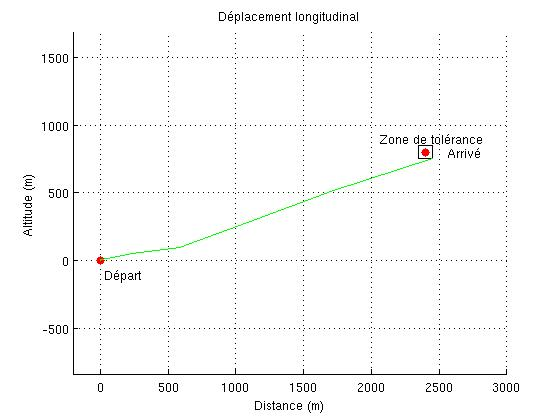
\includegraphics[scale=0.54]{images/resultatCplex1.jpg}
	\caption{Planification de trajectoire sur un monde vide}
	\label{fig:resultatCplex1}
\end{figure}

Ces résultats montrent que notre modélisation d'un problème de planification en CSP fonctionne, nous arrivons à déterminer une séquence de commandes permettant la validation de l'objectif.

Néanmoins plusieurs problèmes persistent, l'ajout d'obstacles modifie grandement le temps de calcul du solveur, la variation du temps de la mission également. Dans le tableau suivant sont représentés différentes configurations : 
\begin{center}
\begin{tabular}{|c|c|c|c|c|}
	\hline stepMax & 11 & 13 & 12 & 12 \\ 
	\hline nombres d'obstacles & 0 & 0 & 0 & 1 \\ 
	\hline altitude objectif (m) & 800 & 800 & 800 & 800 \\ 
	\hline distance objectif (m) & 2400 & 2400 & 5875 & 5875 \\ 
	\hline\hline temps de calcul (s) & 1.08 & 325.42 & 1,46 & 7,66 \\ 
	\hline 
\end{tabular} 
\end{center}

Lors de ces tests il nous ait apparu que le temps de calcul été fortement lié au nombre d'itération maximum (lié au temps de la mission) et à la distance à parcourir.

Il est préférable de régler la variable $stepMax$ en fonction de la distance à parcourir, par exemple en prenant en compte la vitesse moyenne, en effet la distance parcourue dépend uniquement du temps de la mission et de la vitesse $Va$. 

La différence de temps de calcul entre les deux premières simulations vient du fait que la distance à parcourir était trop faible vis à vis du temps de la mission, cela implique une vitesse moyenne faible de l'avion (< 100 m/s), alors que la vitesse nominale de notre aéronef est de 235 m/s.
Pour les mêmes raisons, la troisième simulation présente un temps de calcul relativement faible alors que la distance à parcourir est plus grande.

Dans la dernière simulation nous avons placé un obstacle comme présenté dans la figure \ref{fig:resultatCplex2}, alors que cet obstacle ne figurait pas sur la trajectoire initiale (simulation 3), nous pouvons voir que le temps de calcul a déjà augmenté.

En rajoutant d'autres obstacles, et notamment sur la trajectoire initiale, le temps de calcul explose et nous n'arrivons pas à avoir de solution. Nous supposons que cela est du à un problème de convexité de l'espace de recherche mais nous n'avons pas pu vérifier.

\begin{figure}[h]
	\centering	
	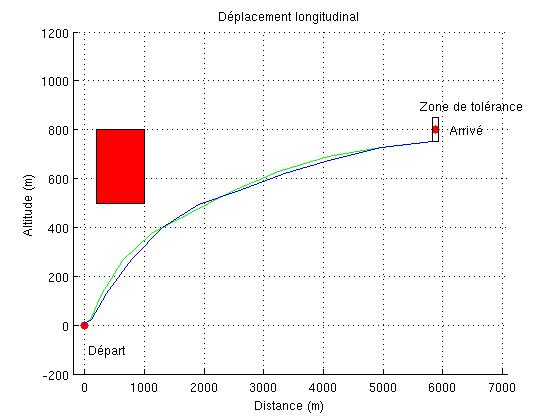
\includegraphics[scale=0.6]{images/resultatCplex2.jpg}
	\caption{Résultat des scénarios 3 (vert) et 4 (bleu)}
	\label{fig:resultatCplex2}
\end{figure}

L'ensemble de ces résultats est encourageant, notre modélisation fonctionne globalement même si des problèmes d'optimisation reste à résoudre. 

\noindent
\shadowbox{\begin{minipage}{\textwidth}
		\textbf{Résumé :} Plusieurs outils ont été testés pour implémenter notre démarche. JaCoP dans un premier temps offre une écriture rapide du problème et des résultats proches de ceux que nous pouvons avoir sur MatLab en terme de précision de calcul sur les espaces d'état. Néanmoins il présente de fortes divergences lors du passage à l'échelle.
		
		Cplex offre un solveur plus performant mais le langage OPL ne nous offre pas assez de possibilité sur l'écriture des variables de types expressions. La librairie JAVA fournie par Cplex semble pouvoir répondre à toute nos attentes, au vue des résultats que nous avons pu avoir, il est nécessaire de se pencher sur l'optimisation de certaines contraintes, ainsi que sur l'utilisation plus avancée du solveur.		
	\end{minipage}}


\chapter{Conclusion et perspectives}
Pour conclure ce rapport je souhaite revenir sur quelques points. 

Le problématique du stage était de définir une démarche permettant de savoir si un aéronef présentant des changements de loi de pilotage (modèle hybride) était capable de réussir une mission donnée. Pour répondre à cette problématique nous avions plusieurs objectifs à atteindre, tout d'abord réussir à trouver le formalisme qui allait nous permettre d'intégrer tous nos composants ensemble (dynamique continue, aspect de mission et de l'environnement). Le formalisme qui a été choisi est celui des CSP, il offre une grande flexibilité de représentation et plusieurs solveurs proposent la prise en compte de variables continues et entières dans un même problème.

Par la suite il s'agissait d'écrire le problème de planification dans ce formalisme, pour cela nous avons traduit les aspects de planification classique (variables, actions, objectifs...) dans le formalisme des CSP. La représentation CSP, très mathématique, nous convenait mais nous étions incapables de savoir si elle allait pouvoir être implémentée et surtout si elle allait permettre de résoudre des problèmes à échelle humaine, c'est à dire des problèmes de planification sur plusieurs heures et kilomètres.

Nous avons donc commencé à lister plusieurs outils à notre disposition et les avons testé. JaCoP nous a permis d'aller assez loin d'un point de vue implémentation et résultat, malheureusement le passage à l'échelle a totalement remis en question notre choix. L'utilisation du solveur Cplex semblait être le meilleur choix, il est plus robuste et présente plusieurs fonctionnalités qu'il nous manquait dans JaCoP (variable expression). Le premier choix pour l'utilisation de Cplex a été d'utiliser le langage de programmation OPL, mais ce langage, bien que très proche des mathématiques et donc d'une représentation CSP, ne permettait pas la définition de variable de manière récursive. Nous avons donc rapidement changé pour passer sur la librairie Cplex pour JAVA. C'est cette approche qui nous a permis d'avoir les meilleurs résultats. Tout n'a pas encore pu être testé mais les résultats sont très encourageants.
%Cette librairie est assez longue à prendre en main, c'est pour cela que pour le moment aucun résultat probant n'a pu être produit.

Même si nous n'avons pas encore réussi à tout implémenter, cela ne remet pas en question notre démarche et notre modélisation pour le moment. Ce travail de stage n'est qu'un préambule à la planification de système hybride. Plusieurs pistes de travail nous sont apparues : 

\begin{itemize}
\item[->] Continuer d'écrire la modélisation avec la librairie JAVA de Cplex qui semble être un très bon candidat;
\item[->] Utiliser MatLab et la libraire Cplex pour MatLab : Plutôt que de simuler l'aéronef via le calcul des espaces d'état (donc modèle linéarisé) et de la dynamique de l'automate hybride, il serait peut-être possible de récupérer les sorties du système directement depuis le modèle non-linéaire simulink de l'aéronef. Cela apporterait plus de précision et de réalité vis à vis de l'aéronef. Donc à chaque instant, on donnerait les commandes (variables de décision) en entrée du simulink, et celui ci nous donnerait les sorties (dans notre exemple Altitude, vitesse et angle).
\item[->] Une autre idée est d'utiliser de la recherche locale. Un outil a été développé à l'ONERA : InCell, nous avons commencé à étudier cet outil pour savoir s'il pourrait convenir à notre problème. L'avantage de la recherche locale est que l'on écrit soi-même les heuristiques de recherches de solution, mais cela implique une moins bonne généralisation et automatisation. En effet la recherche locale s'appuie sur des connaissances expertes de la mission, de l'aéronef etc. Donc il n'est pas assuré que nous arriverions à écrire un problème de recherche locale assez général pour pouvoir être appliquée à n'importe quelle mission et/ou aéronef.
\item[->] Une dernière idée est de ne pas tenter de planifier d'un seul coup toute la mission. Un algorithme classique de recherche de chemin dans un graphe pourrait nous fournir des points de passage (non contraint par la dynamique de l'aéronef), puis ensuite nous appliquerons notre démarche entre chaque point de passage (\cite{chanthery_planification_2005}\cite{dicheva_planification_2012}). Cela pourrait permettre d'éviter les problèmes de passage à l'échelle que nous avons eu avec JaCoP.
\end{itemize}
  
\newpage
\newgeometry{textheight=29.7cm}
  \bibliographystyle{alpha}
  \bibliography{references2}
\addcontentsline{toc}{chapter}{Bibliographie}
  
\end{document}

